\documentclass[a4paper,11pt]{amsart}

% =========================================================================
%  Informe de laboratorio — Práctica 8: Efecto Doppler con ultrasonidos
%  Estilo: artículo científico minimalista (tipografía Palatino, versalitas,
%  enunciados numerados por sección), paleta de azules y grises sobrios.
% =========================================================================

% --- IDIOMA Y CODIFICACIÓN ------------------------------------------------
\usepackage[utf8]{inputenc}
\usepackage[T1]{fontenc}
\usepackage[spanish,es-tabla,es-nodecimaldot]{babel}

% --- TIPOGRAFÍA (Palatino, como el documento de referencia) ---------------
\usepackage{mathpazo}
\linespread{1.05}
\usepackage[final]{microtype}

% --- MATEMÁTICAS Y UNIDADES ------------------------------------------------
\usepackage{amsmath, amssymb, mathtools}
\usepackage{bm}
\usepackage{siunitx}
\sisetup{
  output-decimal-marker = {,},
  group-minimum-digits  = 4,
  group-digits          = integer,
  group-separator       = {\,},
  per-mode              = symbol,
  separate-uncertainty  = true,
  range-phrase          = {\text{ a }},
  detect-all            = false
}

% --- PÁGINA, COLORES Y GRÁFICOS --------------------------------------------
\usepackage[a4paper,margin=2.6cm]{geometry}
\usepackage{graphicx}
\usepackage{xcolor}
\definecolor{azulprof}{HTML}{1B365D}    % azul marino
\definecolor{azulacero}{HTML}{3B6EA8}   % azul acero
\definecolor{azulclaro}{HTML}{B7CBE3}   % azul hielo
\definecolor{grispizarra}{HTML}{5B6770} % gris pizarra
\definecolor{grisclaro}{HTML}{E4E8EC}   % gris perla
\definecolor{azulfondo}{HTML}{F3F7FB}   % fondo tenue de referencias y resultados
\definecolor{acento}{HTML}{B8800A}      % acento sobrio (ámbar oscuro) para comparaciones
\usepackage{tikz}
\usetikzlibrary{babel, arrows.meta, calc, positioning, decorations.pathmorphing,
                decorations.markings, patterns}
\usepackage{pgfplots}
\pgfplotsset{compat=1.17}
\usepackage{booktabs}
\usepackage{multirow}
\usepackage[most]{tcolorbox}
\usepackage{array}
\usepackage{enumitem}
\setlist[itemize]{leftmargin=1.6em, itemsep=2pt, topsep=4pt}
\setlist[enumerate]{leftmargin=1.8em, itemsep=2pt, topsep=4pt}

% --- ENLACES Y REFERENCIAS CRUZADAS ----------------------------------------
\usepackage[colorlinks=true, linkcolor=azulacero, citecolor=azulacero,
            urlcolor=azulacero, plainpages=false, pdfusetitle=false,
            pdftitle={Práctica 8: Efecto Doppler con ultrasonidos},
            pdfauthor={David Gómez García; Daniel Martín Guerrero}]{hyperref}
\usepackage[spanish,nameinlink]{cleveref}

% --- BIBLIOGRAFÍA -----------------------------------------------------------
\usepackage{csquotes}
\usepackage[backend=biber, style=numeric, sorting=none, giveninits=true,
            maxbibnames=6, minbibnames=3, doi=true, url=true,
            isbn=false]{biblatex}
\addbibresource{referencias.bib}
\DeclareFieldFormat[article,techreport,unpublished]{title}{#1\isdot}
\DeclareFieldFormat{url}{\url{#1}}
\renewcommand*{\bibfont}{\small}
\setlength{\bibitemsep}{3pt}

% --- CABECERAS ---------------------------------------------------------------
\pagestyle{headings}
\makeatletter
\def\@evenhead{\small\scshape\thepage\hfil Laboratorio de Mecánica y Ondas\hfil}
\def\@oddhead{\small\scshape\hfil Práctica 8: Efecto Doppler con ultrasonidos\hfil\thepage}
\def\ps@headings{%
  \let\@mkboth\markboth
  \def\@evenhead{\small\scshape\normalfont\thepage\hfil Laboratorio de Mecánica y Ondas}%
  \def\@oddhead{\small\scshape\normalfont Efecto Doppler con ultrasonidos\hfil\thepage}%
  \let\@evenfoot\@empty \let\@oddfoot\@empty}
\makeatother
\numberwithin{equation}{section}
\setcounter{tocdepth}{1}
\makeatletter
\def\@@and{y}
\renewcommand{\keywordsname}{Palabras clave}
\makeatother

% =========================================================================
%               NOTACIÓN Y MACROS DE USO FRECUENTE
% =========================================================================
\newcommand{\vs}{v_{\mathrm{s}}}              % velocidad del sonido
\newcommand{\vst}{\tilde{v}_{\mathrm{s}}}     % valor teórico esperado
\newcommand{\vE}{v_{\mathrm{E}}}              % velocidad del emisor
\newcommand{\vR}{v_{\mathrm{R}}}              % velocidad del receptor
\newcommand{\fE}{f_{\mathrm{E}}}              % frecuencia emitida
\newcommand{\fR}{f_{\mathrm{R}}}              % frecuencia recibida
\newcommand{\TE}{T_{\mathrm{E}}}
\newcommand{\TR}{T_{\mathrm{R}}}
\newcommand{\dif}{\mathrm{d}}
\newcommand{\Tcoef}{t_{95,\nu}}               % factor de cobertura al 95 %
\newcommand{\ext}[1]{U(#1)}                   % incertidumbre ampliada
\newcommand{\mean}[1]{\overline{#1}}
\DeclareMathOperator{\var}{var}
\DeclareMathOperator{\cov}{cov}
% Dato pendiente de incorporar (se resalta con discreción)
\newcommand{\pend}[1]{\textcolor{grispizarra}{\colorbox{grisclaro}{\strut\,#1\,}}}
\newcommand{\pendiente}[1]{\textcolor{grispizarra}{\textit{[#1]}}}

% =========================================================================
%        ENTORNOS FORMALES (enunciados numerados, estilo artículo)
% =========================================================================
\usepackage{amsthm}

% Enunciados en cursiva (resultados generales)
\newtheoremstyle{cienplano}{10pt}{10pt}{\itshape}{}%
  {\bfseries\color{azulprof}}{.}{0.6em}%
  {\thmname{#1}\thmnumber{ #2}\thmnote{\normalfont\upshape\ (#3)}}
% Definiciones, cálculos y estimaciones (cuerpo en redonda)
\newtheoremstyle{ciendef}{10pt}{10pt}{\normalfont}{}%
  {\bfseries\color{azulprof}}{.}{0.6em}%
  {\thmname{#1}\thmnumber{ #2}\thmnote{\normalfont\upshape\ (#3)}}
% Observaciones (encabezado en cursiva)
\newtheoremstyle{cienobs}{8pt}{8pt}{\normalfont}{}%
  {\itshape\color{azulprof}}{.}{0.6em}%
  {\thmname{#1}\thmnumber{ #2}\thmnote{\normalfont\upshape\ (#3)}}

\theoremstyle{cienplano}
\newtheorem{proposicion}{Proposición}[section]
\newtheorem{resultado}[proposicion]{Resultado}
\newtheorem{conclusion}[proposicion]{Conclusión}
\theoremstyle{ciendef}
\newtheorem{hipotesis}[proposicion]{Hipótesis}
\newtheorem{calculo}[proposicion]{Cálculo de incertidumbre}
\newtheorem{estimacion}[proposicion]{Estimación lineal}
\theoremstyle{cienobs}
\newtheorem{observacion}[proposicion]{Observación}

% --- Referencia formalizada --------------------------------------------------
% Caja fina con fondo tenue y título sobre el borde (como las definiciones de
% «Leyes básicas de la electrostática»). Cuerpo en cursiva y, al pie, la fuente
% completa con autor, título y número de cita. Comparte contador con los
% enunciados.  Uso: \begin{referencia}[título]{clave-bib} ... \end{referencia}
\newcounter{referencia}
\renewcommand{\thereferencia}{\theproposicion}
\newtcolorbox{referenciabox}[2]{%
  enhanced, breakable, sharp corners,
  colback=azulfondo, colframe=azulclaro, boxrule=0.4pt,
  left=10pt, right=10pt, top=7pt, bottom=6pt,
  before skip=14pt, after skip=12pt,
  attach boxed title to top left={yshift*=-\tcboxedtitleheight/2, xshift=8pt},
  boxed title style={colback=white, colframe=white, sharp corners, boxrule=0pt,
                     left=3pt, right=3pt, top=1pt, bottom=1pt},
  fonttitle=\bfseries\color{azulprof}, coltitle=azulprof,
  fontupper=\itshape,
  title={Referencia~\thereferencia\ifx\relax#1\relax\else\ \normalfont(#1)\fi},
  after upper={\par\vspace{5pt}{\color{azulclaro}\hrule height 0.4pt}\vspace{4pt}%
    {\upshape\footnotesize\color{grispizarra}\raggedleft
     \citeauthor{#2}, \citetitle{#2}~\cite{#2}.\par}}}
\newenvironment{referencia}[2][]
  {\par\stepcounter{proposicion}\refstepcounter{referencia}\begin{referenciabox}{#1}{#2}}
  {\end{referenciabox}}
\crefname{referencia}{referencia}{referencias}

% --- Método (caja azulada para los fundamentos del tratamiento de datos) -----
\newcounter{metodo}
\renewcommand{\themetodo}{\theproposicion}
\newtcolorbox{metodobox}[1]{%
  enhanced, breakable, sharp corners,
  colback=azulfondo, colframe=azulclaro, boxrule=0.4pt,
  left=10pt, right=10pt, top=7pt, bottom=5pt,
  before skip=14pt, after skip=12pt,
  attach boxed title to top left={yshift*=-\tcboxedtitleheight/2, xshift=8pt},
  boxed title style={colback=white, colframe=white, sharp corners, boxrule=0pt,
                     left=3pt, right=3pt, top=1pt, bottom=1pt},
  fonttitle=\bfseries\color{azulprof}, coltitle=azulprof,
  title={Método~\themetodo\ifx\relax#1\relax\else\ \normalfont(#1)\fi}}
\newenvironment{metodo}[1][]
  {\par\stepcounter{proposicion}\refstepcounter{metodo}\begin{metodobox}{#1}}
  {\end{metodobox}}
\crefname{metodo}{método}{métodos}
\Crefname{metodo}{Método}{Métodos}
\Crefname{referencia}{Referencia}{Referencias}

% --- Resultado destacado ----------------------------------------------------
% Fondo azulado tenue y filete lateral: magnitudes calculadas con su
% incertidumbre.  Uso: \begin{destacado}[rótulo opcional] ... \end{destacado}
\newtcolorbox{destacado}[1][]{%
  enhanced, sharp corners, frame hidden, colback=azulfondo,
  borderline west={1.6pt}{0pt}{azulacero},
  left=10pt, right=8pt, top=2pt, bottom=4pt,
  before skip=8pt, after skip=10pt,
  before upper={\ifx\relax#1\relax\else{\scshape\small\color{azulacero}#1}\par\vspace{-4pt}\fi}}

\crefname{proposicion}{proposición}{proposiciones}
\Crefname{proposicion}{Proposición}{Proposiciones}
\crefname{resultado}{resultado}{resultados}
\crefname{conclusion}{conclusión}{conclusiones}
\crefname{hipotesis}{hipótesis}{hipótesis}
\crefname{calculo}{cálculo}{cálculos}
\crefname{estimacion}{estimación}{estimaciones}
\crefname{observacion}{observación}{observaciones}
\crefname{section}{sección}{secciones}
\Crefname{section}{Sección}{Secciones}
\crefname{subsection}{sección}{secciones}
\Crefname{subsection}{Sección}{Secciones}
\crefname{table}{tabla}{tablas}
\Crefname{table}{Tabla}{Tablas}
\crefname{figure}{figura}{figuras}
\Crefname{figure}{Figura}{Figuras}
\crefname{equation}{ecuación}{ecuaciones}
\Crefname{equation}{Ecuación}{Ecuaciones}
\crefformat{equation}{ecuación~(#2#1#3)}
\Crefformat{equation}{Ecuación~(#2#1#3)}
\crefrangeformat{equation}{ecuaciones~(#3#1#4)--(#5#2#6)}
\crefmultiformat{equation}{ecuaciones~(#2#1#3)}{ y~(#2#1#3)}{, (#2#1#3)}{ y~(#2#1#3)}

% --- Estilo de gráficas de datos (como en «Leyes básicas de la electrostática»)
\pgfplotsset{
  datos/.style={
    tick label style={font=\scriptsize}, label style={font=\small},
    axis lines=left, axis line style={grispizarra},
    grid=major, grid style={grisclaro, line width=0.4pt},
    every tick/.style={grispizarra},
    legend style={font=\scriptsize, draw=none, fill=white, fill opacity=0.9,
                  text opacity=1, cells={anchor=west}},
    legend cell align=left,
    /pgf/number format/use comma, /pgf/number format/1000 sep={\,},
    scaled ticks=false,
  },
  puntoA/.style={only marks, mark=*, mark size=2.1pt, azulprof,
    mark options={fill=azulprof, draw=white, line width=0.3pt},
    error bars/.cd, x dir=both, x explicit, y dir=both, y explicit,
    error bar style={line width=0.6pt, azulprof}, error mark options={rotate=90, mark size=2.2pt, line width=0.6pt, azulprof}},
  puntoB/.style={only marks, mark=square*, mark size=1.9pt, azulacero,
    mark options={fill=azulclaro, draw=azulacero, line width=0.5pt},
    error bars/.cd, x dir=both, x explicit, y dir=both, y explicit,
    error bar style={line width=0.6pt, azulacero}, error mark options={rotate=90, mark size=2.2pt, line width=0.6pt, azulacero}},
  ajuste/.style={azulprof, line width=1.1pt},
  teorica/.style={acento, line width=0.9pt, densely dashed},
}

% Referencia a un panel de figura: «figura 5\,(b)», enlazada en bloque
\newcommand{\figpanel}[2]{\hyperref[#1]{figura~\ref*{#1}\,\textup{(#2)}}}

% Pies de figura y tabla, en la línea del documento de referencia
\usepackage[font=small, labelfont={sc,color=azulprof}, labelsep=period,
            margin=0.6cm, justification=justified]{caption}

% =========================================================================
%                     VARIABLES PARA LA PORTADA
% =========================================================================
\newcommand{\Universidad}{Universidad de Salamanca}
\newcommand{\Facultad}{Facultad de Ciencias}
\newcommand{\Titulacion}{Grado en Física}
\newcommand{\Asignatura}{Laboratorio de Mecánica y Ondas}
\newcommand{\NumPractica}{Práctica 8}
\newcommand{\TituloPractica}{Efecto Doppler\\con ultrasonidos}
\newcommand{\tipotrabajo}{Informe de laboratorio}
\newcommand{\miNombre}{David Gómez García \\ Daniel Martín Guerrero}
\newcommand{\miTutor}{Mario Amado \\ Ivan de Martino \\ Manuel Pino}
\newcommand{\miUbicacion}{Salamanca}

% =========================================================================
%                     DATOS DEL ARTÍCULO (cabecera)
% =========================================================================
\title{Efecto Doppler con ultrasonidos}
\author{David Gómez García}
\author{Daniel Martín Guerrero}
\address{Grado en Física, Facultad de Ciencias, Universidad de Salamanca,
         Salamanca, España}
\date{}



% =========================================================================
%                                DOCUMENTO
% =========================================================================
\begin{document}
% --- PORTADA ----------------------------------------------------------------
\pagenumbering{alph}
%%%%%%%%%%%%%%%%%%%%%%%%%%%%%%%%%%%%%%%%%%%%%%%%%%%%%%%%%%%%%%%%%%%%%%%%
% Portada — estilo artículo científico, motivo: frentes de onda Doppler
% Requiere (definidos en main.tex): colores azulprof, azulacero, azulclaro,
% grispizarra, grisclaro; y las macros \Universidad, \Facultad, \Titulacion,
% \Asignatura, \NumPractica, \TituloPractica, \tipotrabajo, \miNombre,
% \miTutor, \miUbicacion.
%%%%%%%%%%%%%%%%%%%%%%%%%%%%%%%%%%%%%%%%%%%%%%%%%%%%%%%%%%%%%%%%%%%%%%%%

\begin{titlepage}
\thispagestyle{empty}
\pagecolor{white}

\begin{tikzpicture}[remember picture, overlay,
    pg/.style={x=1cm, y=1cm}]
  \coordinate (O) at (current page.south west);

  % ----------------------------------------------------------------
  % Motivo gráfico: frentes de onda de una fuente que se desplaza hacia
  % la derecha (compresión a la derecha, dilatación a la izquierda).
  % ----------------------------------------------------------------
  \begin{scope}
    \clip (O) rectangle ($(O)+(21cm,24.6cm)$);
    \foreach \k in {0,...,15}{
      \pgfmathsetmacro{\cx}{8.2+0.36*\k}
      \pgfmathsetmacro{\rr}{8.4-0.60*\k}
      \pgfmathsetmacro{\pc}{14+5.2*\k}
      \pgfmathsetmacro{\lw}{0.25+0.035*\k}
      \draw[azulprof!\pc!azulclaro, line width=\lw pt]
        ($(O)+(\cx cm,17.2cm)$) circle (\rr cm);
    }
    \fill[azulprof] ($(O)+(8.2cm+0.36cm*15,17.2cm)$) circle (2.2pt);
  \end{scope}

  % ----------------------------------------------------------------
  % Señal con desplazamiento Doppler (chirp): frecuencia creciente
  % ----------------------------------------------------------------
  \begin{scope}[shift={(O)}]
    \draw[azulacero, line width=0.9pt, domain=2.2:18.8, samples=420, smooth]
      plot ({\x}, {12.95 + 0.33*sin(deg((\x-2.2)*(2.2+0.58*(\x-2.2))))});
  \end{scope}

  % ----------------------------------------------------------------
  % Cabecera: logotipos y filete
  % ----------------------------------------------------------------
  \node[anchor=north west, inner sep=0] at ($(O)+(2.2cm,27.9cm)$)
    {
\includegraphics[height=1.42cm]{Logo USAL.png}};
  \node[anchor=north east, inner sep=0] at ($(O)+(18.8cm,27.9cm)$)
    {
\includegraphics[height=1.42cm]{Logo Facultad de Ciencias.png}};
  \draw[grispizarra!60, line width=0.4pt]
    ($(O)+(2.2cm,26.0cm)$) -- ($(O)+(18.8cm,26.0cm)$);
  \node[anchor=north west, inner sep=0, text=grispizarra, font=\scshape\small]
    at ($(O)+(2.2cm,25.75cm)$)
    {\textls[80]{\Universidad\ · \Facultad}};
  \node[anchor=north east, inner sep=0, text=grispizarra, font=\scshape\small]
    at ($(O)+(18.8cm,25.75cm)$)
    {\textls[80]{\Titulacion}};

  % ----------------------------------------------------------------
  % Bloque del título
  % ----------------------------------------------------------------
  \node[anchor=south west, inner sep=0, text=azulacero, font=\scshape\large,
        text width=16.6cm]
    at ($(O)+(2.2cm,11.2cm)$)
    {\textls[120]{\Asignatura\ ·\ \NumPractica}};

  \node[anchor=north west, inner sep=0, text=azulprof, text width=16.6cm,
        align=left]
    at ($(O)+(2.2cm,11.0cm)$)
    {\fontsize{35}{39}\selectfont\bfseries\TituloPractica};

  \draw[azulacero, line width=1.4pt]
    ($(O)+(2.2cm,7.35cm)$) -- ($(O)+(4.7cm,7.35cm)$);

  \node[anchor=north west, inner sep=0, text=grispizarra, text width=16.6cm,
        align=left, font=\itshape\large]
    at ($(O)+(2.2cm,7.05cm)$)
    {$\displaystyle f_{\mathrm{R}} \;=\; f_{\mathrm{E}}\,
      \frac{v_{\mathrm{s}}-v_{\mathrm{R}}}{v_{\mathrm{s}}-v_{\mathrm{E}}}$};

  % ----------------------------------------------------------------
  % Pie: tipo de trabajo, autores, tutores, lugar y fecha
  % ----------------------------------------------------------------
  \draw[grispizarra!60, line width=0.4pt]
    ($(O)+(2.2cm,5.1cm)$) -- ($(O)+(18.8cm,5.1cm)$);

  \node[anchor=north west, inner sep=0, text width=4.6cm, align=left]
    at ($(O)+(2.2cm,4.75cm)$)
    {{\scshape\small\color{azulacero}\textls[80]{Documento}}\\[3pt]
     {\large\bfseries\color{azulprof}\tipotrabajo}};

  \node[anchor=north west, inner sep=0, text width=5.6cm, align=left]
    at ($(O)+(7.2cm,4.75cm)$)
    {{\scshape\small\color{azulacero}\textls[80]{Autores}}\\[3pt]
     {\large\color{black!85}\miNombre}};

  \node[anchor=north west, inner sep=0, text width=5cm, align=left]
    at ($(O)+(13.8cm,4.75cm)$)
    {{\scshape\small\color{azulacero}\textls[80]{Tutores}}\\[3pt]
     {\large\color{black!85}\miTutor}};

  \node[anchor=south east, inner sep=0, text=grispizarra, font=\scshape\small]
    at ($(O)+(18.8cm,1.45cm)$)
    {\textls[100]{\miUbicacion, \number\year}};
  \fill[azulprof] ($(O)+(0,0)$) rectangle ($(O)+(21cm,0.45cm)$);
  \fill[azulacero] ($(O)+(0,0)$) rectangle ($(O)+(7cm,0.45cm)$);
  \fill[azulclaro] ($(O)+(0,0)$) rectangle ($(O)+(3cm,0.45cm)$);
\end{tikzpicture}

\end{titlepage}

\clearpage
\pagenumbering{arabic}
\setcounter{page}{1}

\begin{abstract}
Medimos cómo cambia la frecuencia de un ultrasonido cuando emisor y receptor
se mueven uno respecto del otro sobre un carril. A partir de ese cambio
estimamos la velocidad del sonido en el aire mediante un ajuste lineal y la
comparamos con el valor que predice la temperatura del laboratorio; además,
estimamos la frecuencia de emisión en las dos configuraciones posibles. Los
resultados se expresan con su incertidumbre típica y ampliada al
\SI{95}{\percent}, siguiendo \emph{Notes on Uncertainty in Measurements}.
\end{abstract}

\maketitle
\tableofcontents

% =========================================================================
\newpage
\section{Introducción}
% =========================================================================
La experiencia y su posterior análisis recogidos en este informe presentan
como temática nuclear un fenómeno físico conocido como efecto Doppler.
Consiste en el cambio de frecuencia que percibe un observador cuando él y la
fuente de la onda se mueven uno respecto del otro. Hoy está detrás de la
velocimetría por ultrasonidos, del radar y del corrimiento al rojo de las
galaxias~\cite{TIPLER,HALLIDAY}.

Aquí lo reproducimos a pequeña escala: un emisor y un receptor de
ultrasonidos se mueven uno respecto del otro a velocidad conocida, y
comparamos la frecuencia emitida con la recibida.

\subsection{Objetivos}\label{sec:objetivos}
\begin{itemize}
    \item Hallar la velocidad con la que se propagan ondas ultrasonidos en un medio como el aire.
    \item Evidenciar y calcular las diferencias entre la frecuencia emitida y recibida ante varias situaciones dinámicas del emisor y receptor.
\end{itemize}
La velocidad del sonido la obtenemos como pendiente de un ajuste lineal
(\cref{eq:emisor}) y la contrastamos con su valor teórico; las diferencias
de frecuencia, midiendo $\fE$, $\fR$ y la velocidad relativa $v$ con el emisor
o con el receptor en movimiento.

\subsection{Material empleado}\label{sec:material}
Para el correcto desarrollo del montaje experimental, se ha hecho uso del siguiente instrumental:
\begin{itemize}
    \item Unidad de emisión y detección de ultrasonidos.
    \item Carril y coche autopropulsado.
    \item Emisor, receptor y soportes.
    \item Barrera fotoeléctrica y temporizador.
    \item Ordenador y unidad de medida Cobra-3.
\end{itemize}

\subsection{Montaje experimental}\label{sec:montaje}
Emisor y receptor se enfrentan sobre el eje de un carril; uno queda fijo y el
otro viaja sobre el coche autopropulsado, de modo que la recta que los une
coincide con la dirección del movimiento (\cref{fig:montaje}). Una barrera
fotoeléctrica, hacia la mitad del recorrido, mide la velocidad del coche
cuando la cruza, y es en ese instante cuando se registra la frecuencia
recibida. Ambas señales llegan al ordenador a través de la unidad
Cobra-3~\cite{GUION-P8}.

\begin{figure}[ht]
\centering
\begin{tikzpicture}[>=Stealth, x=1cm, y=1cm, font=\small]
  % --- carril ---
  \fill[grisclaro] (0,0) rectangle (13.2,0.26);
  \draw[grispizarra, line width=0.6pt] (0,0) rectangle (13.2,0.26);
  \foreach \x in {0.6,1.2,...,12.6}{\draw[grispizarra!50, line width=0.3pt] (\x,0)--(\x,0.26);}
  % --- coche ---
  \begin{scope}[shift={(2.2,0.26)}]
    \draw[azulprof, fill=azulclaro!55, line width=0.7pt, rounded corners=1.5pt]
      (0,0.16) rectangle (2.5,0.78);
    \draw[azulprof, fill=white, line width=0.7pt] (0.5,0.16) circle (0.16);
    \draw[azulprof, fill=white, line width=0.7pt] (2.0,0.16) circle (0.16);
    % soporte y emisor
    \draw[grispizarra, line width=0.9pt] (1.25,0.78) -- (1.25,1.35);
    \draw[azulprof, fill=azulacero!85, line width=0.7pt]
      (1.25,1.35) -- ++(0.07,0.07) -- ++(0,0.46) -- ++(-0.14,0) -- ++(0,-0.46) -- cycle;
    \fill[azulprof] (1.31,1.60) circle (0.05);
    \node[azulprof, anchor=south] at (1.25,2.0) {emisor $(\mathrm{E})$};
    % velocidad
    \draw[->, line width=0.9pt, azulprof] (-0.05,1.1) -- (-0.85,1.1);
    \node[azulprof, anchor=east] at (-0.9,1.1) {$\vE$};
  \end{scope}
  % --- ondas emitidas ---
  \foreach \r/\o in {0.45/90, 0.85/70, 1.25/50, 1.65/35}{
    \draw[azulacero, opacity=0.35+\o/200, line width=0.7pt]
      (3.55,1.86) ++(-32:\r) arc[start angle=-32, end angle=32, radius=\r];
  }
  % --- receptor fijo ---
  \begin{scope}[shift={(11.0,0.26)}]
    \draw[grispizarra, line width=0.9pt] (0,0) -- (0,1.35);
    \draw[azulprof, fill=azulacero!85, line width=0.7pt]
      (0,1.35) -- ++(-0.07,0.07) -- ++(0,0.46) -- ++(0.14,0) -- ++(0,-0.46) -- cycle;
    \node[azulprof, anchor=south] at (0,2.0) {receptor $(\mathrm{R})$};
    \draw[grispizarra, fill=grisclaro, line width=0.6pt] (-0.4,0) rectangle (0.4,0.12);
  \end{scope}
  % --- barrera fotoeléctrica ---
  \begin{scope}[shift={(7.0,0.26)}]
    \draw[grispizarra, line width=1pt] (-0.45,0) -- (-0.45,1.05);
    \draw[grispizarra, line width=1pt] (0.45,0) -- (0.45,1.05);
    \fill[azulprof] (-0.45,0.95) circle (0.07);
    \fill[azulprof] (0.45,0.95) circle (0.07);
    \draw[azulacero, densely dashed, line width=0.6pt] (-0.45,0.95) -- (0.45,0.95);
    \node[azulprof, align=center, anchor=south] at (0,1.15)
      {barrera\\fotoeléctrica};
  \end{scope}
  % --- acotación de la distancia de propagación ---
  \draw[|<->|, grispizarra, line width=0.5pt] (3.7,-0.55) -- (11.0,-0.55)
    node[midway, fill=white, inner sep=1.5pt, text=black!80] {línea de propagación};
  % --- interfaz y ordenador ---
  \draw[azulprof, fill=azulclaro!55, line width=0.7pt, rounded corners=2pt]
    (5.6,-2.35) rectangle (8.0,-1.45);
  \node[azulprof, align=center] at (6.8,-1.9) {unidad\\Cobra-3};
  \draw[azulprof, fill=white, line width=0.7pt, rounded corners=2pt]
    (9.5,-2.45) rectangle (12.6,-1.45);
  \node[azulprof, align=center] at (11.05,-1.95) {ordenador\\PHYWE Measure};
  \draw[->, line width=0.8pt, azulprof] (8.0,-1.9) -- (9.5,-1.95);
  % --- conexiones (cables) ---
  \draw[grispizarra, densely dotted, line width=0.8pt]
    (7.0,0.26) -- (7.0,-1.45);
  \draw[grispizarra, densely dotted, line width=0.8pt]
    (11.0,0.26) .. controls (11.0,-0.9) and (8.4,-0.9) .. (8.0,-1.7);
  \draw[grispizarra, densely dotted, line width=0.8pt]
    (3.45,0.26) .. controls (3.45,-1.0) and (5.4,-1.0) .. (5.6,-1.8);
\end{tikzpicture}
\caption{Esquema de nuestro montaje experimental. El emisor, solidario al coche
autopropulsado, se mueve con velocidad $\vE$ a lo largo del carril; el
receptor permanece fijo (en la segunda configuración intercambiamos sus
posiciones). La barrera fotoeléctrica
permite medir la velocidad del coche, y la unidad Cobra-3 adquiere tanto esa
velocidad como la frecuencia recibida y las transfiere al ordenador. Las
líneas de puntos representan las conexiones eléctricas.}
\label{fig:montaje}
\end{figure}


% =========================================================================
\section{Fundamentos teóricos}\label{sec:fundamentos}
% =========================================================================
\begin{referencia}[Efecto Doppler]{FV6-ECJ}\label{ref:doppler}
{El efecto Doppler es un fenómeno físico que describe el cambio en la frecuencia percibida de una onda cuando la fuente emisora de la onda y el observador están en movimiento relativo 
entre sí. Este cambio de frecuencia no se debe a una modificación real de la frecuencia de la 
onda emitida, sino a un cambio en la forma en que el observador percibe la onda debido al 
movimiento. 
La causa del efecto Doppler radica en la compresión o dilatación de las ondas debida al 
movimiento relativo entre la fuente y el observador. Si la fuente se mueve hacia el 
observador, las ondas se comprimen, lo que resulta en una longitud de onda más corta y una 
frecuencia percibida más alta. Si la fuente se aleja, las ondas se dilatan, lo que resulta en una 
longitud de onda más larga y una frecuencia percibida más baja. El efecto Doppler se aplica 
a cualquier tipo de onda, incluyendo ondas sonoras, ondas de luz, ondas de agua, etc.}

{Si la fuente se acerca al observador ($\vE>0$), la longitud de onda se acorta y la frecuencia se hace mayor. En ondas de sonido se aprecia una frecuencia más aguda. Por el contrario, si el emisor se aleja del receptor ($\vE<0$), la longitud de onda 
aparente es mayor y la frecuencia menor. El sonido se hace más grave.}
\end{referencia}

La \cref{fig:frentes}
lo ilustra para una fuente $\mathrm{S}$ que se desplaza con velocidad
$\vE>0$: los frentes se amontonan por delante y se separan por detrás, de modo
que $\mathrm{R}_2$ percibe una frecuencia mayor que la emitida y
$\mathrm{R}_1$ una menor.

\begin{figure}[ht]
\centering
\begin{tikzpicture}[>=Stealth, scale=0.85, every node/.style={scale=0.9}]
  \definecolor{cS}{HTML}{1B365D}
  \definecolor{cA}{HTML}{7A8C9E}
  \definecolor{cB}{HTML}{3B6EA8}
  % ---------- Panel izquierdo: frentes espaciales ----------
  \begin{scope}
    \node[anchor=west, text=grispizarra] at (-5.6,3.9) {\small\scshape (a)\; frentes de onda};
    \draw[->, line width=0.7pt, grispizarra] (-5.5,0) -- (4.6,0) node[right, text=black] {$x$};
    \def\rA{3.8} \def\cA{0}
    \def\rB{2.8} \def\cB{0.7}
    \def\rC{1.8} \def\cC{1.4}
    \def\rD{0.8} \def\cD{2.1}
    \foreach \c/\r/\o in {\cA/\rA/45,\cB/\rB/60,\cC/\rC/75,\cD/\rD/90}{
      \draw[cB!\o!cA, line width=0.9pt] (\c,0) circle (\r);}
    \foreach \c/\n in {\cA/0,\cB/1,\cC/2,\cD/3}{
      \fill[cS] (\c,0) circle (2.3pt) node[below=3pt, text=cS] {$x_{\n}$};}
    \node[text=cS, above=11pt, fill=white, inner sep=1.5pt] at (\cD,0) {$\mathrm{S}$};
    \fill[cB] (-4.7,0) circle (3pt) node[below=4pt, text=cB, fill=white, inner sep=1.5pt] {$\mathrm{R}_1$};
    \fill[cB] (4.15,0) circle (3pt) node[below=4pt, text=cB, fill=white, inner sep=1.5pt] {$\mathrm{R}_2$};
    \draw[->, dashed, grispizarra] (\cA,0) -- ++(110:\rA)
      node[midway, left=2pt, fill=white, inner sep=1pt, text=black!80] {$r_0$};
    \draw[->, dashed, grispizarra] (\cB,0) -- ++(80:\rB)
      node[midway, right=1pt, fill=white, inner sep=1pt, text=black!80] {$r_1$};
    \draw[->, dashed, grispizarra] (\cC,0) -- ++(125:\rC)
      node[midway, left=1pt, fill=white, inner sep=1pt, text=black!80] {$r_2$};
    \draw[->, dashed, grispizarra] (\cD,0) -- ++(55:\rD)
      node[midway, right=1pt, fill=white, inner sep=1pt, text=black!80] {$r_3$};
    \draw[->, line width=0.9pt, cS] (\cD-0.6,-1.7) -- ++(1.2,0)
      node[midway, below=1pt] {$\vE$};
    \node[anchor=west, align=left, text=black!80] at (-5.7,2.45)
      {$r_k=\vs\,(t-t_k)$};
    \node[anchor=west, align=left, text=black!80] at (-5.7,-2.45)
      {$x_k=\vE\,t_k$};
  \end{scope}
  % ---------- Panel derecho: señales ----------
  \begin{scope}[shift={(6.6,0)}]
    \def\w{5.5} \def\ha{1.1}
    \node[anchor=west, text=grispizarra] at (0,3.9) {\small\scshape (b)\; señales temporales};
    \foreach \y/\col/\lab/\f/\st in {2.55/cS/{\mathrm{S}}/1.5/0,
                                     0/cB/{\mathrm{R}_1}/0.9/1.8,
                                     -2.55/cB/{\mathrm{R}_2}/2.5/0.8}{
      \begin{scope}[shift={(0,\y)}]
        \draw[grisclaro, line width=0.4pt, step=0.5] (0,-\ha) grid (\w,\ha);
        \draw[->, line width=0.7pt, grispizarra] (0,0) -- (\w+0.45,0);
        \draw[->, line width=0.7pt, grispizarra] (0,-\ha-0.2) -- (0,\ha+0.2);
        \draw[\col, line width=0.9pt] (0,0) -- (\st,0);
        \draw[\col, line width=0.9pt, domain=\st:\w, samples=160]
          plot (\x, {0.85*sin((\x-\st)*180*\f)});
        \node[\col, fill=white, inner sep=2.5pt, draw=\col!60, line width=0.4pt]
          at (\w-0.45,\ha-0.2) {$\lab$};
      \end{scope}}
    \node[text=black!80, anchor=north] at (\w/2,-3.9) {tiempo $t$};
  \end{scope}
\end{tikzpicture}
\caption{Efecto Doppler generado por una fuente $\mathrm{S}$ que se desplaza
con velocidad $\vE$. (a)~Frentes de onda emitidos en distintos instantes:
compresión en el sentido del movimiento y dilatación en el opuesto.
(b)~Señal emitida frente a las percibidas por los receptores $\mathrm{R}_1$
(menor frecuencia) y $\mathrm{R}_2$ (mayor frecuencia), desfasadas por el
tiempo de propagación. Esquema cualitativo, sin escala.}
\label{fig:frentes}
\end{figure}
\begin{figure}[ht]
\centering
\begin{tikzpicture}[>=Stealth, scale=1.15]
  \draw[->, line width=0.5pt, grispizarra!60] (-2,0) -- (10,0)
    node[right, text=grispizarra] {$x$};
  \draw[azulacero, line width=0.9pt, densely dashed, domain=-1.5:1, samples=60]
    plot (\x,{sin(\x*180)});
  \draw[azulacero, line width=0.9pt, densely dashed, domain=7:9.5, samples=60]
    plot (\x,{sin(\x*180)});
  \draw[azulprof, line width=1.4pt, domain=1:7, samples=180]
    plot (\x,{sin(\x*180)});
  \foreach \x/\t in {1/emisor,7/receptor}{
    \draw[grispizarra!70, densely dotted, line width=0.8pt] (\x,-1.4) -- (\x,1.4);
    \node[draw=grispizarra!50, fill=white, inner sep=3.5pt, text=azulprof,
          font=\small\scshape] at (\x,1.75) {\t};}
  \draw[->, line width=0.9pt, azulprof] (1,-1.75) -- (0,-1.75)
    node[midway, below] {$\vE-\vs$};
  \draw[->, line width=0.9pt, azulprof] (7,-1.75) -- (6,-1.75)
    node[midway, below] {$\vR-\vs$};
  \draw[grispizarra!60, line width=0.4pt] (2.5,1.05) -- (2.5,1.55);
  \draw[grispizarra!60, line width=0.4pt] (4.5,1.05) -- (4.5,1.55);
  \draw[|<->|, line width=0.7pt, azulacero] (2.5,1.4) -- (4.5,1.4)
    node[midway, fill=white, inner sep=2pt, above=-1pt] {$\lambda$};
\end{tikzpicture}
\caption{Movimientos del emisor y del receptor en el sistema de referencia
de la onda, para $\vs>\vE,\vR$. Se toma como sentido positivo de propagación
el de izquierda a derecha; ambas velocidades relativas son negativas.}
\label{fig:relativo}
\end{figure}

Para cuantificarlo, supongamos que el medio está en reposo y que emisor y
receptor se mueven a lo largo de la recta que los une con velocidades
constantes $\vE$ y $\vR$ respecto al medio (positivas en el sentido de
propagación), siendo $\vs>\vE,\vR$ la velocidad de la onda. En el sistema de
referencia de la onda (\cref{fig:relativo}) el emisor recorre una longitud de
onda $\lambda$ en un tiempo $\TE$ y el receptor en un tiempo $\TR$, de modo que
\begin{equation}\label{eq:lambda}
  \lambda=\TE\,(\vs-\vE)=\TR\,(\vs-\vR),
  \qquad\Longrightarrow\qquad
  \frac{\fR}{\fE}=\frac{\TE}{\TR}=\frac{\vs-\vR}{\vs-\vE}.
\end{equation}
Con la velocidad relativa $v\equiv\vE-\vR$ (positiva si emisor y receptor se
acercan) resulta
\begin{equation}\label{eq:doppler}
  \fR=\fE\left(1+\frac{v}{\vs-\vE}\right).
\end{equation}
En el laboratorio se estudian dos casos particulares.

\textbf{Emisor móvil y receptor en reposo} ($v=\vE$):
\begin{equation}\label{eq:emisor}
  \fR=\frac{\fE}{1-v/\vs}
  \qquad\Longleftrightarrow\qquad
  v=\vs\left(1-\frac{\fE}{\fR}\right),
\end{equation}
una relación lineal entre $v$ y $1-\fE/\fR$ cuya pendiente es la velocidad del
sonido.

\textbf{Emisor en reposo y receptor móvil} ($v=-\vR$):
\begin{equation}\label{eq:receptor}
  \fR=\fE\left(1+\frac{v}{\vs}\right)
  =\frac{\fE}{1-v/\vs}-\fE\,\frac{(v/\vs)^{2}}{1-v/\vs}.
\end{equation}
Para $|v/\vs|\ll1$ ambos casos coinciden a primer orden y solo difieren en el
término cuadrático de la \cref{eq:receptor}, cuya observabilidad se analiza al
final del informe.

La \cref{fig:cuadratico} compara ambas leyes.

\begin{figure}[ht]
\centering
\pgfplotsset{
  doppler/.style={
    width=0.40\textwidth, height=5.4cm, tick label style={font=\scriptsize},
    label style={font=\small}, axis lines=left, axis line style={grispizarra},
    grid=major, grid style={grisclaro, line width=0.4pt}, every tick/.style={grispizarra},
    legend style={font=\scriptsize, draw=none, fill=white, fill opacity=0.85,
                  text opacity=1, at={(0.03,0.97)}, anchor=north west},
    xlabel={$x=v/\vs$}, xmin=-0.3, xmax=0.3, xtick={-0.3,-0.15,0,0.15,0.3}}}
\begin{tikzpicture}
  \begin{axis}[doppler, ylabel={$\fR/\fE$}, ymin=0.6, ymax=1.5]
    \addplot[azulprof, line width=1pt, domain=-0.3:0.3, samples=100] {1/(1-x)};
    \addplot[azulacero, line width=1pt, dashed, domain=-0.3:0.3, samples=2] {1+x};
    \legend{emisor móvil \eqref{eq:emisor},receptor móvil \eqref{eq:receptor}}
  \end{axis}
\end{tikzpicture}\hfill
\begin{tikzpicture}
  \begin{axis}[doppler, ylabel={$\bigl(\fR-\fE/(1-x)\bigr)/\fE$}, ymin=-0.14, ymax=0.01,
               scaled y ticks=false, yticklabel style={/pgf/number format/fixed,
               /pgf/number format/precision=2}]
    \addplot[azulprof, line width=1pt, domain=-0.3:0.3, samples=100] {-x^2/(1-x)};
    \addplot[grispizarra, line width=0.7pt, densely dashed, domain=-0.3:0.3, samples=2] {0};
  \end{axis}
\end{tikzpicture}
\caption{Emisor móvil frente a receptor móvil. (Izquierda) $\fR/\fE$ en función
de $x=v/\vs$. (Derecha) Diferencia relativa entre ambas leyes, igual a
$-x^{2}/(1-x)$ y nula para el emisor móvil por construcción. El rango de $x$ se
ha ampliado con fines ilustrativos; en el laboratorio $|x|\ll1$.}
\label{fig:cuadratico}
\end{figure}

% =========================================================================
\newpage
\section{Procedimiento experimental}\label{sec:procedimiento}
% =========================================================================
Con el programa PHYWE Measure se mide la velocidad del coche (modo
«Temporizador») y la frecuencia recibida (modo «Contador»), ambas al cruzar
la barrera. Con emisor móvil y receptor en reposo se mide primero $\fE$ en
reposo (al menos seis veces) y después, para tres velocidades del coche y
ambos sentidos de marcha, seis medidas de $v$ y de $\fR$ en cada caso. Luego se
intercambian emisor y receptor y se repite el proceso~\cite{GUION-P8}.

Como la experiencia recogida en este informe se ha desarrollado a lo largo de una mañana, hemos creído preciso tomar dos medidas de temperatura: al inicio y al final de la experiencia. De este modo, podremos garantizar que la velocidad del sonido obtenida a partir de una regresión lineal se sitúe en un rango de valores teóricos.

Dichas temperaturas corresponden a $T_{\mathrm{ini}}=\SI{22,1}{\celsius}$ y $T_{\mathrm{fin}}=\SI{23,5}{\celsius}$.
A fin de determinar el
valor teórico o valor esperado de la velocidad del sonido en el aire,
$\vst$:
\begin{equation}\label{eq:vs}
  \vst = \SI{331,3}{\meter\per\second}\,\sqrt{1+\frac{T}{\SI{273,15}{}}}.
\end{equation}

\subsection{Tratamiento de incertidumbres}\label{sec:incertidumbres}
Seguimos la \emph{Guide to the expression of uncertainty in
measurement}~\cite{GUM}, tal como se recoge en las notas del
laboratorio~\cite{NUM-ARG}. Para una magnitud $y=f(x_1,\dots,x_N)$ con
entradas no correlacionadas, la incertidumbre típica se propaga como
\begin{equation}\label{eq:propagacion}
  u^{2}(y)=\sum_{k=1}^{N}\left(\frac{\partial f}{\partial x_k}\right)^{\!2}u^{2}(x_k),
\end{equation}
y la incertidumbre ampliada al $\SI{95}{\percent}$ es $\ext{y}=t_{95,\nu}\,u(y)$,
con $t_{95,\nu}$ el factor de cobertura de Student para $\nu$ grados de
libertad~\cite{NUM-ARG}; el resultado se expresa como $y\pm\ext{y}$.
Las incertidumbres se dan con una sola cifra significativa, salvo cuando la
primera es un 1, en cuyo caso se conservan dos; el valor se redondea a la
misma posición decimal~\cite{ERR-MP}.

\begin{calculo}[Lectura de la temperatura]\label{calc:T}
Obtenida la lectura de temperatura, $T$, con una resolución del termómetro
$\Delta=\SI{0,1}{\celsius}$, se procede a calcular la incertidumbre asociada a
dicha medida:
\begin{equation}\label{eq:uT}
  \sigma^{2}=\frac{\Delta^{2}}{12}
  \;\longrightarrow\;
  u(T)=\frac{\Delta}{\sqrt{12}}\approx\SI{0,03}{\celsius}.
\end{equation}
En consecuencia, los registros térmicos al comienzo y al final de la experiencia han sido, respectivamente,
\begin{destacado}
\vspace{-6pt}
\begin{equation*}
  T_{\mathrm{ini}}=(\num{22,10}\pm\num{0,03})\,\si{\celsius},
  \qquad
  T_{\mathrm{fin}}=(\num{23,50}\pm\num{0,03})\,\si{\celsius}.
\end{equation*}
\end{destacado}
\end{calculo}

\begin{calculo}[Velocidad esperada del sonido]\label{calc:vs}
Determinar la incertidumbre asociada a cada lectura de la temperatura es un paso
clave antes de poder hallar por propagación la incertidumbre propia de $\vst$.
Por la \cref{eq:propagacion},
\begin{equation*}
  u^{2}(\vst)=\left(\frac{\partial\vst}{\partial T}\right)^{\!2}u^{2}(T).
\end{equation*}
Para calcular la derivada parcial nos apoyamos en la dependencia térmica de
la \cref{eq:vs}:
\begin{equation}\label{eq:dvsdT}
  \frac{\partial\vst}{\partial T}
  =\frac{331{,}3}{2\cdot273{,}15\,\sqrt{1+T/273{,}15}}
  =\frac{331{,}3}{546{,}3\,\sqrt{1+T/273{,}15}}.
\end{equation}
Sustituyendo este resultado, evaluado en la temperatura medida, y calculando
la raíz cuadrada,
\begin{equation}\label{eq:uvs}
  u(\vst)=\left|\frac{\partial\vst}{\partial T}\right|\frac{\SI{0,1}{\kelvin}}{\sqrt{12}}
  \approx
  \begin{cases}
    \num{0,5833}\,\si{\meter\per\second\per\kelvin}\cdot\SI{0,0289}{\kelvin}=\SI{0,017}{\meter\per\second} & (T_{\mathrm{ini}}),\\[2pt]
    \num{0,5819}\,\si{\meter\per\second\per\kelvin}\cdot\SI{0,0289}{\kelvin}=\SI{0,017}{\meter\per\second} & (T_{\mathrm{fin}}).
  \end{cases}
\end{equation}
Luego, se espera que la velocidad del sonido en el aire para las condiciones inicial y final
en las que se ha encontrado el laboratorio sea
\begin{destacado}
\vspace{-6pt}
\begin{equation*}
  \vst^{\,\mathrm{ini}}=(\num{344,442}\pm\num{0,017})\,\si{\meter\per\second},
  \qquad
  \vst^{\,\mathrm{fin}}=(\num{345,257}\pm\num{0,017})\,\si{\meter\per\second}.
\end{equation*}
\end{destacado}
Observamos que la velocidad del sonido al final de la mañana es mayor que al principio. Esto es coherente con que la temperatura haya aumentado, ya que la velocidad del sonido en el aire aumenta con la temperatura.

Como la temperatura varió de forma gradual durante la mañana, en el análisis
tomamos como valor de referencia el punto medio de ambos, asignándole una
distribución uniforme entre ellos, $u^{2}=(\Delta\vst)^{2}/12+u^{2}(\vst^{\,\mathrm{ini}})$:
\begin{destacado}[Valor de referencia]
\begin{equation}\label{eq:vsref}
  \vst=(\num{344,9}\pm\num{0,2})\,\si{\meter\per\second}
  \quad(\text{incertidumbre típica}).
\end{equation}
\end{destacado}
\begin{observacion}[Sobre el modelo uniforme]\label{obs:uniforme}
Este procedimiento supone que es razonable representar la variación ambiental
mediante una distribución uniforme entre los dos extremos medidos. Se trata de
una \emph{elección de modelo} para cuantificar la incertidumbre (una evaluación no estadística o «de tipo B» \cite{NUM-ARG}), no de una afirmación de que la temperatura haya
seguido exactamente una distribución uniforme a lo largo de la mañana.
\end{observacion}
\end{calculo}
\subsection{Frecuencia de la señal en reposo}
Antes de abordar las situaciones de movimiento relativo, se ha medido la frecuencia de la onda ultrasonido, enfrentando emisor y receptor, ambos en reposo y situando el emisor acoplado al móvil, justo en la barrera fotoeléctrica, de tal modo que al presionar espacio en el ordenador hemos obtenido valores de 40607 y 40608 Hz para las seis medidas realizadas.

En concreto, las seis lecturas fueron 40607, 40607, 40608, 40608, 40608 y
40608~Hz. Tratamos esta serie estadísticamente (evaluación «de tipo A» ~\cite{NUM-ARG,ERR-MP}) y le añadimos la contribución de la
resolución del contador, $\Delta f=\SI{1}{\hertz}$.

\begin{calculo}[Frecuencia de emisión en reposo]\label{calc:fE}
La media y la desviación típica muestrales de las $n=6$ lecturas son
\begin{equation}\label{eq:fEmedia}
  \mean{f}_{\mathrm{E}}=\frac{1}{n}\sum_{i=1}^{n}f_{\mathrm{E},i}=\SI{40607,667}{\hertz},
  \qquad
  s=\sqrt{\frac{1}{n-1}\sum_{i=1}^{n}\bigl(f_{\mathrm{E},i}-\mean{f}_{\mathrm{E}}\bigr)^{2}}=\SI{0,516}{\hertz}.
\end{equation}
La incertidumbre típica de la media (tipo~A) y la debida a la resolución
(tipo~B, distribución uniforme de anchura $\Delta f$) son
\begin{equation}\label{eq:fEuAuB}
  u_{A}=\frac{s}{\sqrt{n}}=\SI{0,211}{\hertz},
  \qquad
  u_{B}=\frac{\Delta f}{\sqrt{12}}=\SI{0,289}{\hertz},
\end{equation}
que se combinan cuadráticamente, con un número efectivo de grados de libertad
dado por la fórmula de Welch--Satterthwaite~\cite{NUM-ARG}:
\begin{equation}\label{eq:fEu}
  u(\fE)=\sqrt{u_{A}^{2}+u_{B}^{2}}=\SI{0,357}{\hertz},
  \qquad
  \nu_{\mathrm{eff}}=(n-1)\,\frac{u^{4}(\fE)}{u_{A}^{4}}\approx41.
\end{equation}
\begin{destacado}
\begin{equation}\label{eq:fE}
  \fE=(\num{40607,7}\pm\num{0,4})\,\si{\hertz}
  \quad(\text{incertidumbre típica}),
\end{equation}
{\small y, con $t_{95,41}=\num{2,02}$, una incertidumbre ampliada al
\SI{95}{\percent} $\ext{\fE}=\SI{0,7}{\hertz}$.}
\end{destacado}
\end{calculo}
\subsection{Medidas de velocidad y frecuencia}
Antes de mostrar los datos obtenidos experimentalmente, es necesario determinar el criterio de signos empleado en cada situación.
Para el caso en el que el emisor es móvil y se enfrenta a un receptor en reposo, tomamos como sentido positivo de movimiento el que se da de derecha a izquierda, es decir, cuando el emisor se acerca al receptor, pues dicha dirección es la de la propagación de la onda ultrasonido. Cuando el emisor se aleje del receptor, dicho movimiento diremos que tendrá sentido negativo.

A fin de ser coherentes con este análisis, en el caso del receptor móvil enfrentado a un emisor en reposo, tomaremos como sentido positivo del movimiento aquel en el que el receptor se aleja del emisor (de izquierda a derecha), pues la onda ultrasonido se propaga en dicha dirección.
La \cref{fig:fotos} muestra el selector mecánico de velocidad y el interruptor
de sentido del móvil. Cada combinación de posición del selector y sentido de
marcha da lugar a seis medidas de la velocidad y otras seis de la frecuencia
recibida.

\begin{figure}[ht]
\centering
\begin{minipage}[b]{0.32\textwidth}\centering
  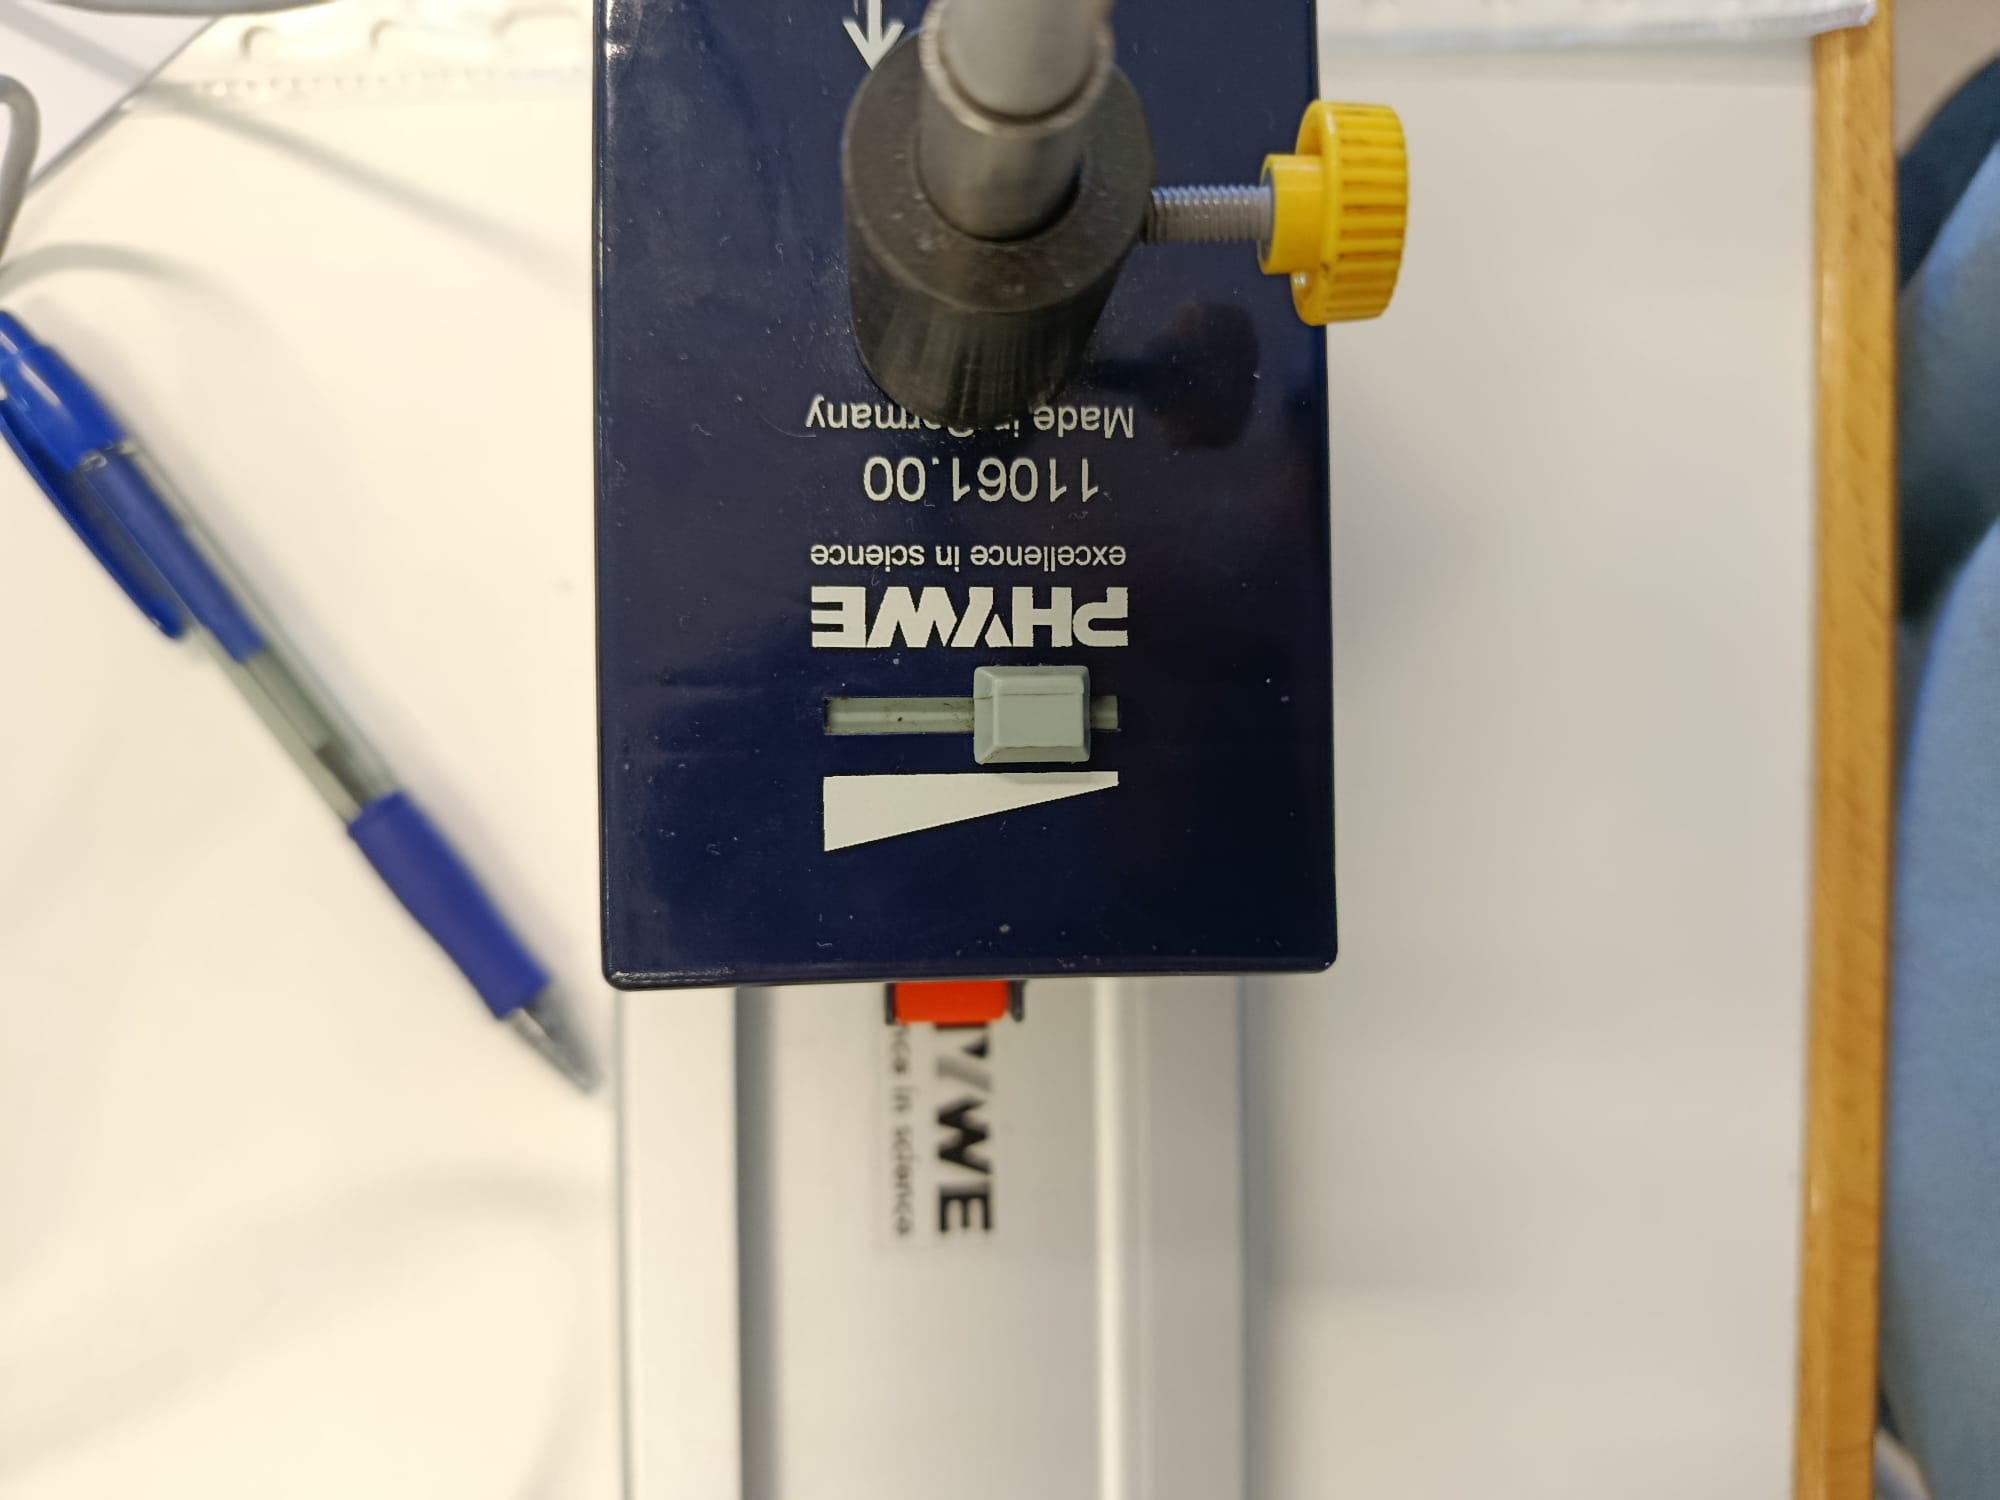
\includegraphics[width=\linewidth]{ima/selector_minima.jpeg}\\[2pt]
  {\small\scshape (a)\; selector: mínima}
\end{minipage}\hfill
\begin{minipage}[b]{0.32\textwidth}\centering
  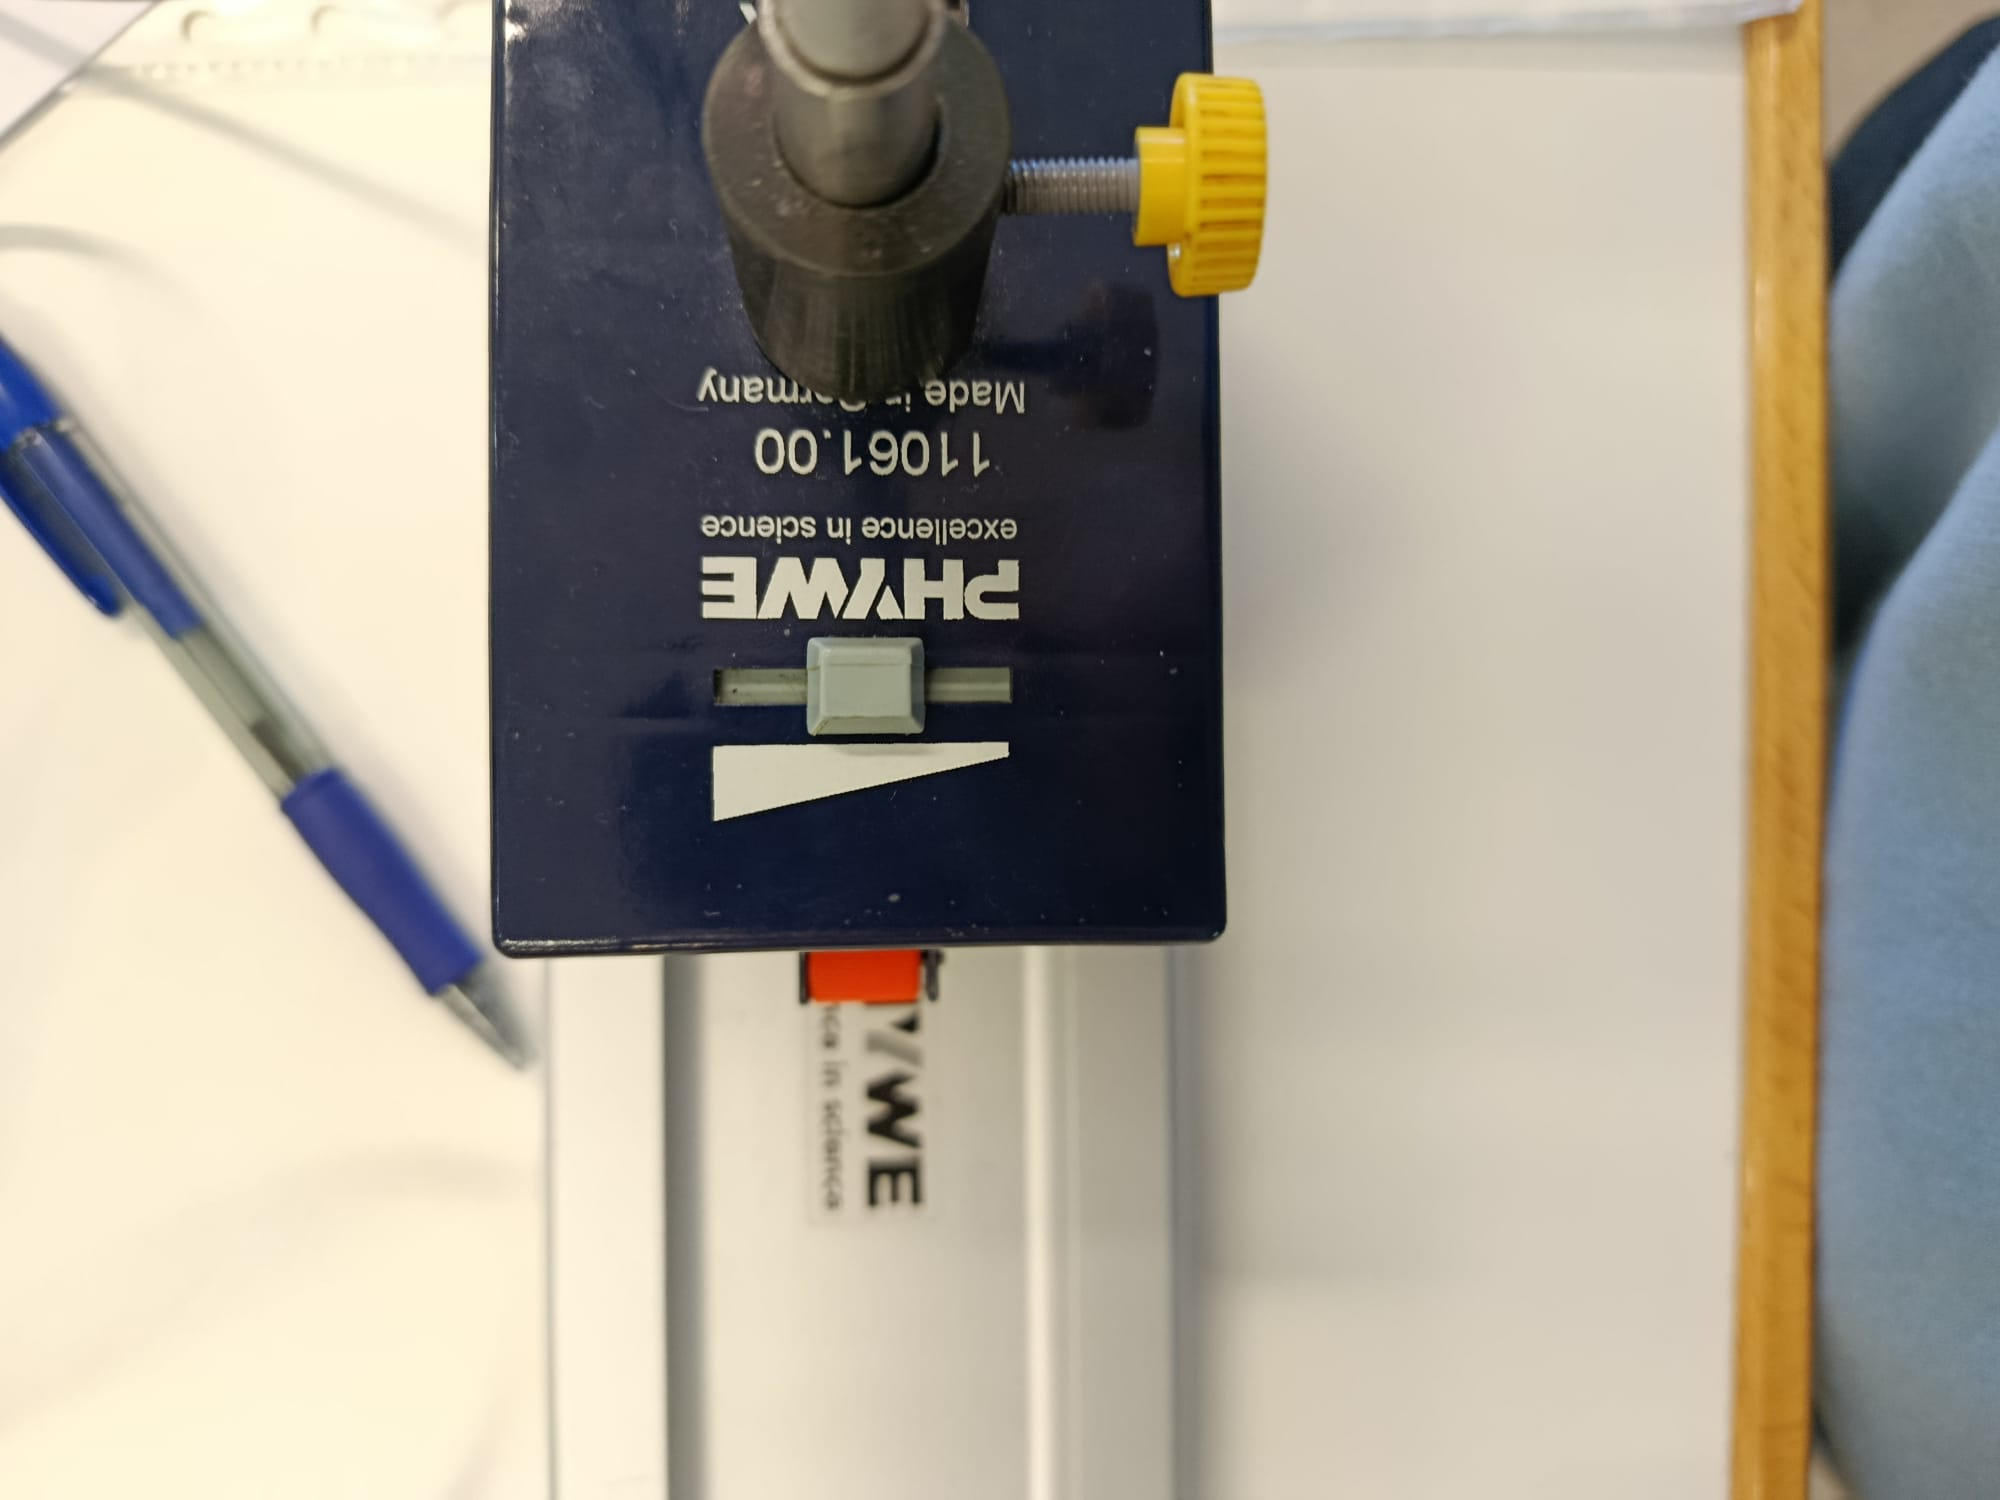
\includegraphics[width=\linewidth]{ima/selector_media.jpeg}\\[2pt]
  {\small\scshape (b)\; selector: media}
\end{minipage}\hfill
\begin{minipage}[b]{0.32\textwidth}\centering
  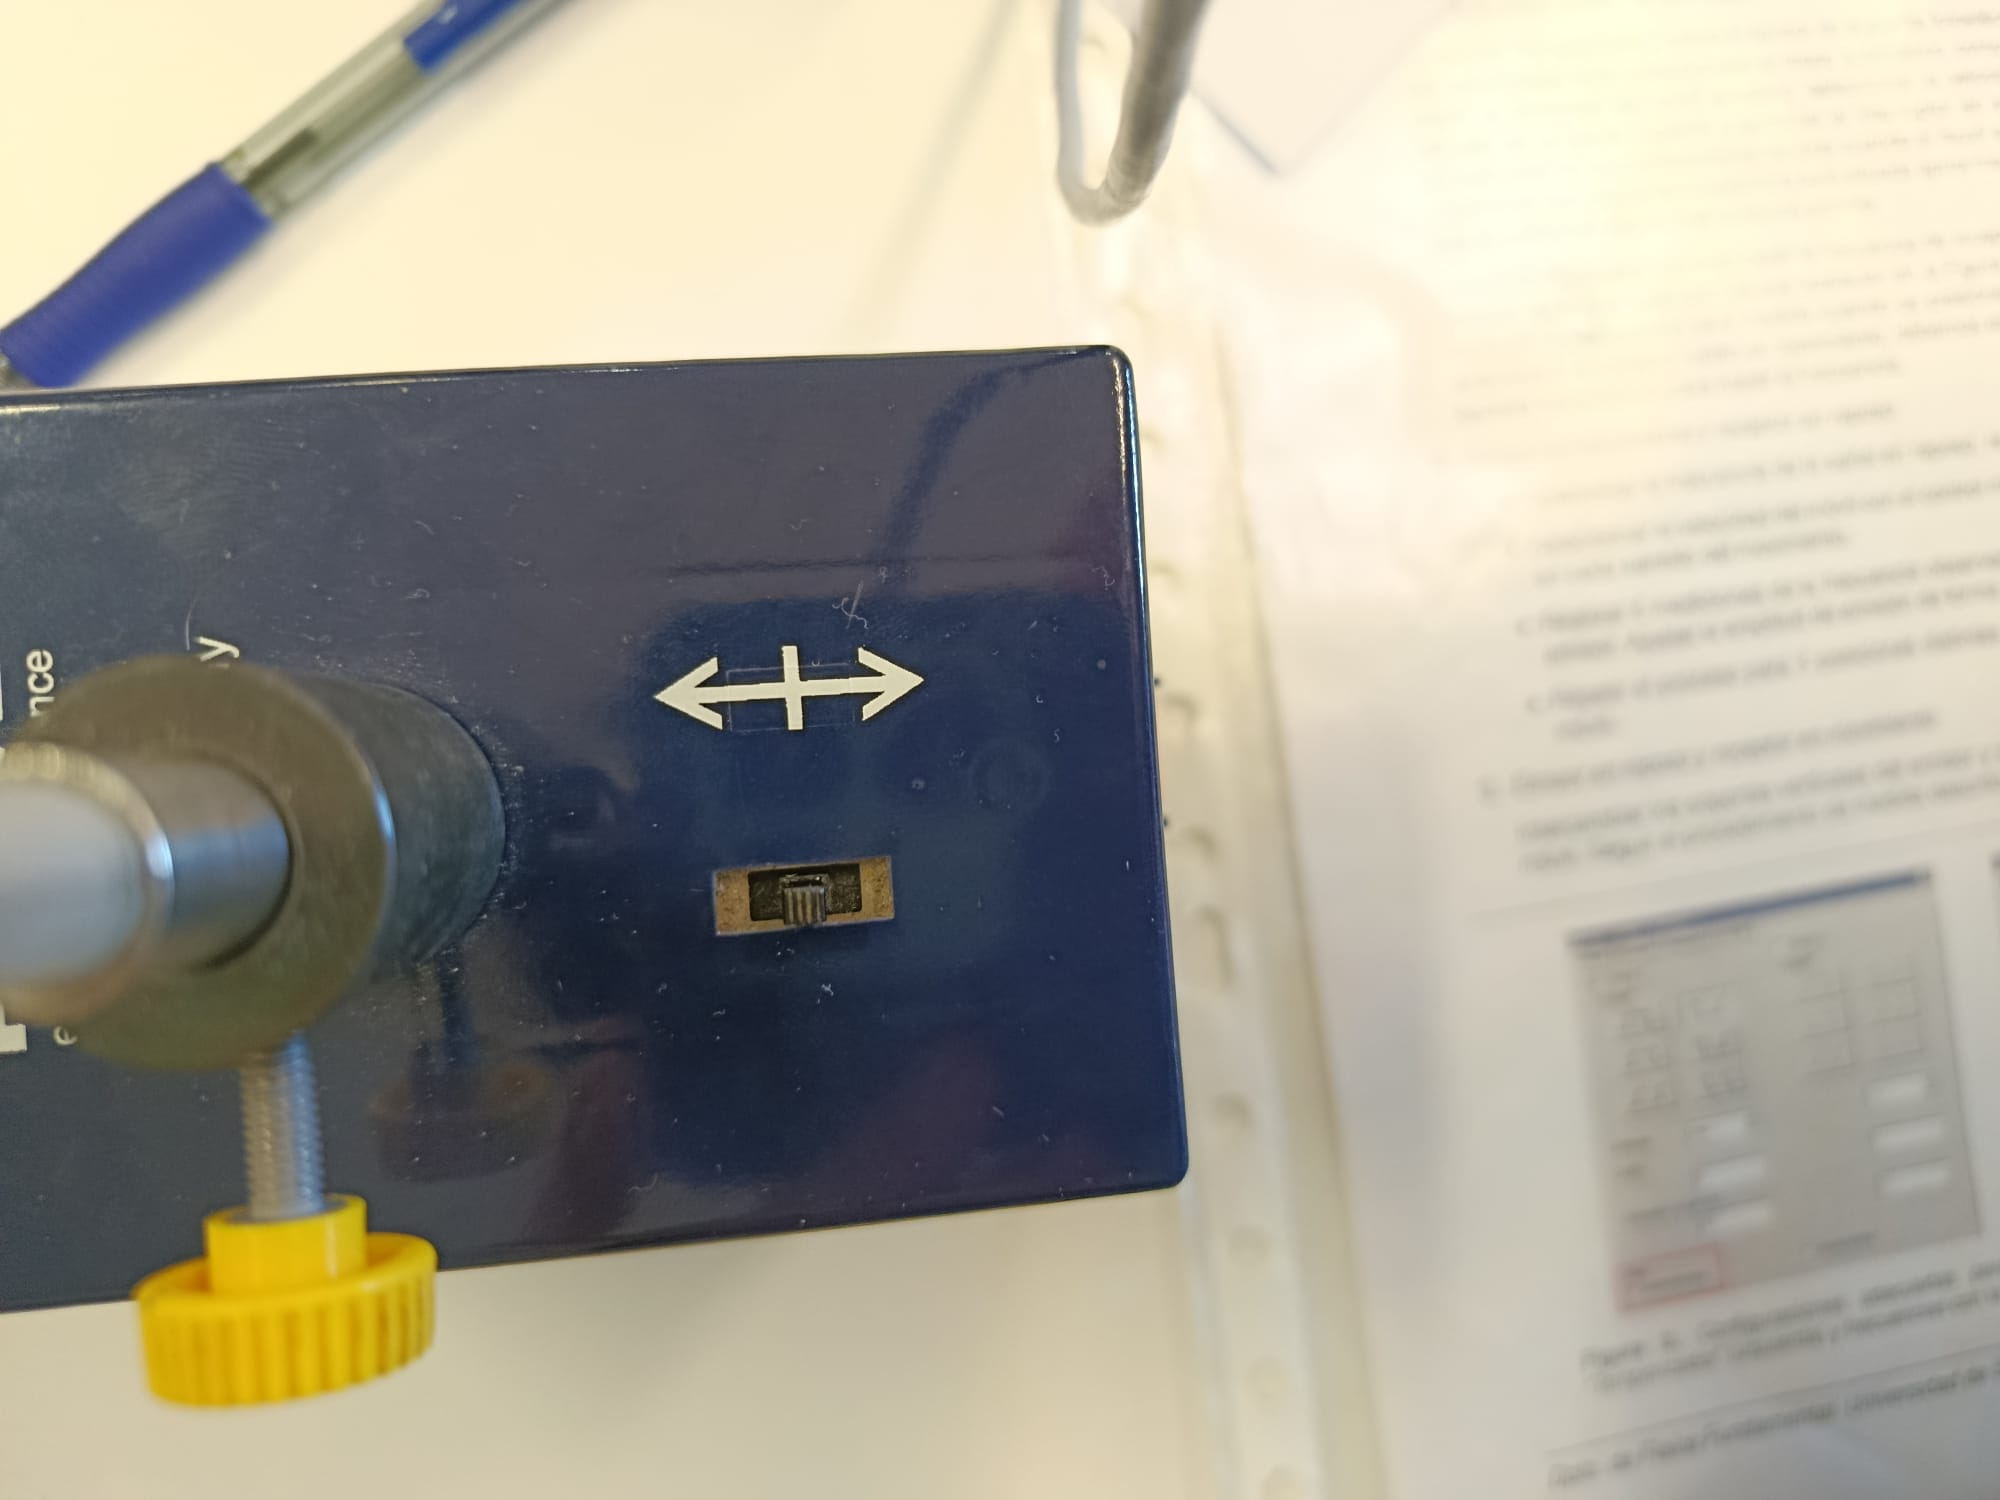
\includegraphics[width=\linewidth]{ima/sentido_mov.jpeg}\\[2pt]
  {\small\scshape (c)\; sentido de marcha}
\end{minipage}
\caption{Controles del móvil. (a,~b)~Posiciones mínima y media del selector
mecánico de velocidad. (c)~Interruptor que invierte el sentido de la marcha.}
\label{fig:fotos}
\end{figure}

\subsubsection{Emisor en movimiento y receptor en reposo}
Tras realizar las medidas de la velocidad en ambos sentidos del movimiento, y
para cada una de las tres posiciones del control mecánico de la velocidad del
móvil, agrupamos los datos en la \cref{tab:datosE}, junto con las frecuencias
recogidas para ambos sentidos del movimiento y para cada posición.

\begin{table}[ht]
\centering
\caption{Medidas directas con el \emph{emisor en movimiento} y el receptor en
reposo. Sentido positivo: el emisor se acerca al receptor. Resoluciones:
$\Delta v=\SI{0,001}{\meter\per\second}$ y $\Delta f=\SI{1}{\hertz}$.}
\label{tab:datosE}
\small
\setlength{\tabcolsep}{5pt}
\renewcommand{\arraystretch}{1.12}
\begin{tabular}{@{}ll*{6}{c}@{}}
\toprule
Selector & Sentido & \multicolumn{6}{c}{Medida $i$}\\
\cmidrule(l){3-8}
 & & 1 & 2 & 3 & 4 & 5 & 6\\
\midrule
\multicolumn{8}{@{}l}{\textit{Velocidad del móvil, $\lvert v_i\rvert$ (\si{\meter\per\second})}}\\[2pt]
Máxima & Positivo & 0,341 & 0,358 & 0,354 & 0,358 & 0,354 & 0,354\\
Máxima & Negativo & 0,381 & 0,388 & 0,382 & 0,382 & 0,380 & 0,382\\
Media & Positivo & 0,227 & 0,222 & 0,226 & 0,222 & 0,223 & 0,225\\
Media & Negativo & 0,241 & 0,240 & 0,240 & 0,244 & 0,244 & 0,243\\
Mínima & Positivo & 0,127 & 0,128 & 0,127 & 0,127 & 0,128 & 0,126\\
Mínima & Negativo & 0,127 & 0,129 & 0,131 & 0,127 & 0,128 & 0,128\\
\midrule
\multicolumn{8}{@{}l}{\textit{Frecuencia recibida, $f_{\mathrm{R},i}$ (\si{\hertz})}}\\[2pt]
Máxima & Positivo & 40699 & 40708 & 40705 & 40703 & 40677 & 40686\\
Máxima & Negativo & 40452 & 40346 & 40382 & 40293 & 40428 & 40265\\
Media & Positivo & 40655 & 40664 & 40657 & 40661 & 40652 & 40656\\
Media & Negativo & 40601 & 40587 & 40586 & 40586 & 40595 & 40590\\
Mínima & Positivo & 40635 & 40642 & 40652 & 40627 & 40629 & 40627\\
Mínima & Negativo & 40608 & 40607 & 40605 & 40601 & 40603 & 40601\\
\bottomrule
\end{tabular}
\end{table}

\subsubsection{Emisor en reposo y receptor en movimiento}
De nuevo, mostramos los resultados experimentales organizados en una tabla
(\cref{tab:datosR}), tanto para las velocidades como para las frecuencias, pero
teniendo en cuenta en este caso que el sentido positivo del movimiento ahora es
de izquierda a derecha.

\begin{table}[ht]
\centering
\caption{Medidas directas con el emisor en reposo y el \emph{receptor en
movimiento}. Sentido positivo: el receptor se aleja del emisor. Resoluciones:
$\Delta v=\SI{0,001}{\meter\per\second}$ y $\Delta f=\SI{1}{\hertz}$.}
\label{tab:datosR}
\small
\setlength{\tabcolsep}{5pt}
\renewcommand{\arraystretch}{1.12}
\begin{tabular}{@{}ll*{6}{c}@{}}
\toprule
Selector & Sentido & \multicolumn{6}{c}{Medida $i$}\\
\cmidrule(l){3-8}
 & & 1 & 2 & 3 & 4 & 5 & 6\\
\midrule
\multicolumn{8}{@{}l}{\textit{Velocidad del móvil, $\lvert v_i\rvert$ (\si{\meter\per\second})}}\\[2pt]
Máxima & Negativo & 0,350 & 0,351 & 0,349 & 0,347 & 0,342 & 0,344\\
Máxima & Positivo & 0,378 & 0,381 & 0,374 & 0,368 & 0,365 & 0,369\\
Media & Negativo & 0,234 & 0,228 & 0,229 & 0,226 & 0,227 & 0,226\\
Media & Positivo & 0,250 & 0,251 & 0,251 & 0,253 & 0,251 & 0,252\\
Mínima & Negativo & 0,136 & 0,140 & 0,139 & 0,140 & 0,139 & 0,140\\
Mínima & Positivo & 0,147 & 0,146 & 0,145 & 0,145 & 0,146 & 0,150\\
\midrule
\multicolumn{8}{@{}l}{\textit{Frecuencia recibida, $f_{\mathrm{R},i}$ (\si{\hertz})}}\\[2pt]
Máxima & Negativo & 40799 & 40720 & 40733 & 40800 & 40676 & 40708\\
Máxima & Positivo & 40429 & 40520 & 40438 & 40500 & 40557 & 40489\\
Media & Negativo & 40655 & 40663 & 40660 & 40662 & 40654 & 40670\\
Media & Positivo & 40582 & 40584 & 40588 & 40588 & 40583 & 40583\\
Mínima & Negativo & 40637 & 40649 & 40652 & 40646 & 40637 & 40642\\
Mínima & Positivo & 40596 & 40611 & 40599 & 40598 & 40598 & 40610\\
\bottomrule
\end{tabular}
\end{table}

\begin{observacion}[Velocidad relativa]\label{obs:signos}
En el análisis empleamos siempre la velocidad relativa $v=\vE-\vR$ de la
\cref{sec:fundamentos}, positiva cuando emisor y receptor se acercan. Con
emisor móvil, $v=\vE$ y su signo coincide con el sentido de las tablas; con el receptor móvil y el emisor en reposo, el alejamiento en el sentido positivo del eje implica \(v_R>0\), por lo que la velocidad relativa definida como \(v=v_E-v_R\) es negativa.
\end{observacion}

\newpage

\subsection{Estimación lineal}\label{sec:ajuste}
Las tres cuestiones del análisis se resuelven ajustando una recta $y=ax+b$ por
mínimos cuadrados. Antes de dar las fórmulas, conviene escribir cada relación
teórica de la \cref{sec:fundamentos} en esa forma e identificar qué papel desempeña
cada magnitud.

\subsubsection{Linealización de los tres casos}

\textbf{Caso 1: emisor móvil, ajuste de la velocidad relativa.} Con el receptor
en reposo, la velocidad relativa es $v=\vE$ y la ley de Doppler queda
\begin{equation*}
  \frac{\fR}{\fE}=\frac{\vs}{\vs-v}
  \qquad\Longrightarrow\qquad
  v=\vs\left(1-\frac{\fE}{\fR}\right).
\end{equation*}
Es una recta cuyas ordenada, pendiente y abscisa son
\begin{equation}\label{eq:lin1}
  \underbrace{v}_{y}=\underbrace{\vs}_{a}\,
  \underbrace{\left(1-\frac{\fE}{\fR}\right)}_{x}+\underbrace{0}_{b}.
\end{equation}
Su pendiente proporciona una estimación experimental de la velocidad del sonido.

\textbf{Caso 2: emisor móvil, ajuste de la frecuencia recibida.} Partiendo de
la misma ecuación y dividiendo numerador y denominador por $\vs$,
$\fR=\fE\,(1-v/\vs)^{-1}$. Si en la abscisa empleamos la velocidad del sonido de
referencia $\vst$ (\cref{eq:vsref}),
\begin{equation}\label{eq:lin2}
  \underbrace{\fR}_{y}=\underbrace{\fE}_{a}\,
  \underbrace{\left(1-\frac{v}{\vst}\right)^{-1}}_{x}+\underbrace{0}_{b},
\end{equation}
y la pendiente estima la frecuencia emitida.

\textbf{Caso 3: receptor móvil, ajuste de la frecuencia recibida.} Con el
emisor en reposo, $v=-\vR$ y la \cref{eq:receptor} se escribe directamente como
\begin{equation}\label{eq:lin3}
  \underbrace{\fR}_{y}=\underbrace{\fE}_{a}\,
  \underbrace{\left(1+\frac{v}{\vst}\right)}_{x}+\underbrace{0}_{b},
\end{equation}
de nuevo con la frecuencia emitida como pendiente. La \cref{tab:ajustes}
resume las tres linealizaciones.

\begin{table}[ht]
\centering
\caption{Linealizaciones empleadas; en todas la ordenada $b$ debe ser compatible con cero.}
\label{tab:ajustes}
\small
\renewcommand{\arraystretch}{1.3}
\begin{tabular}{@{}lllccc@{}}
\toprule
Caso & Configuración & Ordenada $y$ & Abscisa $x$ & Pendiente $a$ & Ordenada $b$\\
\midrule
1 & Emisor móvil & $v$ & $1-\fE/\fR$ & $\vs$ & $0$\\
2 & Emisor móvil & $\fR$ & $(1-v/\vst)^{-1}$ & $\fE$ & $0$\\
3 & Receptor móvil & $\fR$ & $1+v/\vst$ & $\fE$ & $0$\\
\bottomrule
\end{tabular}
\end{table}

\subsubsection{La ordenada en el origen}
Las tres relaciones teóricas tienen la forma $y=ax$: el modelo predice $b=0$.
El ajuste, sin embargo, deja libre la ordenada, y su valor experimental nos servirá
de control.

Si el intervalo $b\pm\ext{b}$ contiene el cero, por ejemplo
$b=(\num{0,2}\pm\num{0,5})\,\si{\hertz}$, la ordenada es \emph{compatible con
cero} y los datos son coherentes con el modelo. Si no lo contiene, por ejemplo
$b=(\num{3,0}\pm\num{0,5})\,\si{\hertz}$, el resultado es difícil de reconciliar
con $b=0$ y apunta a un error sistemático o accidental que hayamos podido cometer en el laboratorio, un problema de calibración o a que el
modelo no describe adecuadamente los datos. Por eso en la práctica insistimos en
comprobar esta condición.

\subsubsection{Ajuste por mínimos cuadrados}
Con $n$ pares $(x_i,y_i)$, incertidumbre común en $y_i$ y despreciable en
$x_i$~\cite{NUM-ARG},
\begin{equation}\label{eq:ajuste}
\begin{gathered}
  a=\frac{\cov(x,y)}{\var(x)},\qquad b=\mean{y}-a\,\mean{x},\qquad
  s_\varepsilon=\sqrt{\frac{\sum_i(y_i-ax_i-b)^{2}}{n-2}},\\[4pt]
  u(a)=\frac{s_\varepsilon}{\sqrt{(n-1)\var(x)}},\qquad
  u(b)=u(a)\sqrt{\mean{x^{2}}},
\end{gathered}
\end{equation}
con $\nu=n-2$ grados de libertad, de modo que $\ext{a}=t_{95,\nu}\,u(a)$.

Las expresiones anteriores suponen que todos los puntos son igual de fiables y
que la abscisa no tiene error. En el primer ajuste no se cumple ninguna de las
dos condiciones: la incertidumbre de cada punto, $u^{2}=s^{2}/n+\Delta^{2}/12$,
varía de \SI{1,3}{\hertz} a \SI{30}{\hertz} en $\fR$, y la abscisa $1-\fE/\fR$,
que hereda la incertidumbre de las frecuencias, es la variable con más error.
Por eso completamos el ajuste con los tres elementos siguientes.

\begin{metodo}[Mínimos cuadrados ponderados]\label{met:pesos}
Cada punto recibe un peso $w_i=1/u_i^{2}$, de forma que los más precisos
influyen más en la recta. Minimizando $\chi^{2}=\sum_iw_i(y_i-ax_i-b)^{2}$ se
obtiene~\cite{NUM-ARG}
\begin{equation}\label{eq:ajustepesos}
\begin{gathered}
  a=\frac{\langle xy\rangle-\langle x\rangle\langle y\rangle}{\langle x^{2}\rangle-\langle x\rangle^{2}},\qquad
  b=\langle y\rangle-a\langle x\rangle,\\[4pt]
  u(a)=\frac{1}{\sqrt{\sum_i w_i}\,\sqrt{\langle x^{2}\rangle-\langle x\rangle^{2}}},\qquad
  u(b)=u(a)\sqrt{\langle x^{2}\rangle},
\end{gathered}
\end{equation}
donde $\langle\cdot\rangle$ denota la media ponderada con los pesos $w_i$.
\end{metodo}

\begin{metodo}[Varianza efectiva]\label{met:vareff}
La abscisa también procede de magnitudes medidas. Un error horizontal
$\delta x$ equivale, sobre la recta, a uno vertical $a\,\delta x$; sumando ambas
contribuciones como varianzas independientes, cada punto queda caracterizado por
\begin{equation}\label{eq:vareff}
  u_i^{2}=u^{2}(y_i)+a^{2}u^{2}(x_i),
\end{equation}
que es la que entra en los pesos. Como depende de la propia pendiente, el
cálculo se itera: un primer ajuste sin la incertidumbre de $x$ da una pendiente
provisional, con ella se recalculan los pesos y se repite hasta que los
resultados apenas cambian.
\end{metodo}

\begin{metodo}[Bondad del ajuste]\label{met:chi2}
El mínimo de $\chi^{2}$ se compara con los grados de libertad,
$\nu=n-2$~\cite{NUM-ARG}. Si $\chi^{2}\approx\nu$, la dispersión de los puntos es
coherente con sus incertidumbres; si $\chi^{2}\gg\nu$, los puntos se apartan de
la recta más de lo esperado, lo que delata errores sistemáticos o incertidumbres
que hemos subestimado. En ese caso, cuando el \emph{chi-cuadrado reducido}
$\chi^{2}/\nu$ es claramente mayor que la unidad, multiplicamos las
incertidumbres de los parámetros por $\sqrt{\chi^{2}/\nu}$~\cite{HUGHES}.
\end{metodo}

La abscisa del primer ajuste hereda la incertidumbre de las frecuencias,
\begin{equation}\label{eq:ux}
  u^{2}\!\left(1-\frac{\fE}{\fR}\right)=\frac{u^{2}(\fE)}{\fR^{2}}+\frac{\fE^{2}\,u^{2}(\fR)}{\fR^{4}},
\end{equation}
y, para estudiar el término cuadrático, la diferencia
$\Delta f=\fR-\fE\,(1-v/\vst)^{-1}$ tiene, con $x\equiv v/\vst$,
\begin{equation}\label{eq:udf}
  u^{2}(\Delta f)=u^{2}(\fR)+\frac{u^{2}(\fE)}{(1-x)^{2}}
  +\frac{\fE^{2}}{\vst^{2}(1-x)^{4}}\Bigl[u^{2}(v)+x^{2}u^{2}(\vst)\Bigr].
\end{equation}

% =========================================================================
\newpage
\section{Análisis de datos y resultados}\label{sec:analisis}
% =========================================================================
\subsection{Emisor en movimiento y receptor en reposo}
Con los datos de las velocidades y las frecuencias, vamos a tomar los valores
medios y a representar los resultados. La \cref{tab:mediasE} recoge la velocidad
media y la frecuencia media registradas para cada sentido del movimiento y para
cada posición del control mecánico, junto con la abscisa del primer ajuste.

\begin{table}[ht]
\centering
\caption{Valores medios con el emisor en movimiento (incertidumbres típicas,
$u^{2}=s^{2}/n+\Delta^{2}/12$). La velocidad relativa $v$ lleva el signo del
sentido de marcha.}
\label{tab:mediasE}
\small
\renewcommand{\arraystretch}{1.25}
\begin{tabular}{@{}llccc@{}}
\toprule
Selector & Sentido & $v$ (\si{\meter\per\second}) & $\mean{f}_{\mathrm{R}}$ (\si{\hertz}) & $10^{3}\,(1-\fE/\fR)$\\
\midrule
Máxima & Positivo & \num{0,353 +- 0,003} & \num{40696 +- 5} & \num{2,18 +- 0,12}\\
Máxima & Negativo & \num{-0,3825 +- 0,0012} & \num{40360 +- 30} & \num{-6,1 +- 0,8}\\
Media & Positivo & \num{0,2242 +- 0,0009} & \num{40657,5 +- 1,8} & \num{1,23 +- 0,04}\\
Media & Negativo & \num{-0,2420 +- 0,0008} & \num{40591 +- 2} & \num{-0,41 +- 0,06}\\
Mínima & Positivo & \num{0,1272 +- 0,0004} & \num{40635 +- 4} & \num{0,68 +- 0,10}\\
Mínima & Negativo & \num{-0,1283 +- 0,0007} & \num{40604,2 +- 1,3} & \num{-0,09 +- 0,03}\\
\bottomrule
\end{tabular}
\end{table}

\textbf{Velocidad del sonido.} La \cref{fig:ajuste1} representa $v$ frente a
$1-\fE/\fR$. Si se cumple la ley de Doppler, los puntos deben alinearse sobre
una recta que pasa por el origen y cuya pendiente es la velocidad del sonido
(\cref{eq:lin1}). Las barras horizontales, que proceden de las frecuencias, son
las dominantes, de ahí que el ajuste use la varianza efectiva
(\cref{met:vareff}).

\begin{figure}[ht]
\centering
\begin{tikzpicture}
  \begin{axis}[datos, name=principal, width=0.86\textwidth, height=6.6cm,
      xmin=-1, xmax=2.6, ymin=-0.45, ymax=0.45, clip=true,
      xlabel={}, xticklabels={}, ylabel={$v$ (\si{\meter\per\second})},
      legend pos=north west, ytick={-0.4,-0.2,0,0.2,0.4},
      yticklabel style={/pgf/number format/fixed, /pgf/number format/precision=1}]
    \addplot[teorica, domain=-1:2.6, samples=2] {0.34485*x};
    \addlegendentry{$v=\vst\,x$ (valor teórico)}
    \addplot[ajuste, domain=-1:2.6, samples=2] {0.2446553*x+(-0.1014381)};
    \addlegendentry{ajuste ponderado}
    \addplot[puntoA] coordinates {(2.17874,0.35317) +- (0.12257,0.00258) (1.22569,0.22417) +- (0.04482,0.00092) (0.68085,0.12717) +- (0.10117,0.00042)};
    \addlegendentry{acercamiento}
    \addplot[puntoB] coordinates {(-0.41471,-0.24200) +- (0.06189,0.00083) (-0.08620,-0.12833) +- (0.03217,0.00068)};
    \addlegendentry{alejamiento}
    \draw[-{Stealth[length=5pt]}, azulacero, line width=0.8pt]
      (axis cs:-0.55,-0.3825) -- (axis cs:-0.97,-0.3825);
    \node[azulacero, font=\scriptsize, anchor=west, align=left]
      at (axis cs:-0.53,-0.3825) {máxima, alejamiento:\\ $10^{3}x=\num{-6,11}$, fuera de escala};
  \end{axis}
  \begin{axis}[datos, at={(principal.south west)}, anchor=north west, yshift=-4pt,
      width=0.86\textwidth, height=3.2cm, xmin=-1, xmax=2.6, ymin=-5, ymax=8.5,
      xlabel={$10^{3}\,x=10^{3}\,(1-\fE/\fR)$}, ylabel={$r_i/u_i$},
      ytick={-3,0,3,6}]
    \addplot[grispizarra, line width=0.5pt, densely dashed, domain=-1:2.6, samples=2] {0};
    \addplot[only marks, mark=*, mark size=1.7pt, azulprof,
      error bars/.cd, y dir=both, y explicit,
      error bar style={line width=0.5pt, azulprof}, error mark options={rotate=90, mark size=1.8pt, azulprof}]
      coordinates {(2.17874,-2.6060) +- (0,1) (1.22569,2.3389) +- (0,1) (-0.41471,-2.5786) +- (0,1) (0.68085,2.5059) +- (0,1) (-0.08620,-0.7351) +- (0,1)};
    \draw[-{Stealth[length=5pt]}, azulacero, line width=0.8pt]
      (axis cs:-0.55,6.602) -- (axis cs:-0.97,6.602);
    \node[azulacero, font=\scriptsize, anchor=west] at (axis cs:-0.53,6.602) {$r/u=\num{6,6}$};
  \end{axis}
\end{tikzpicture}
\caption{Velocidad relativa del emisor frente a $1-\fE/\fR$. Círculos:
acercamiento; cuadrados: alejamiento; barras: incertidumbre típica. Recta
continua: ajuste ponderado con los seis puntos; discontinua: predicción con
$\vst$. El punto de alejamiento a velocidad máxima, fuera de la ventana, se
señala con una flecha. Debajo, los residuos normalizados $r_i/u_i$.}
\label{fig:ajuste1}
\end{figure}

Un ajuste sin pesos (\cref{eq:ajuste}) daría
$\vs=(\num{0,8}\pm\num{0,7})\times10^{2}\,\si{\meter\per\second}$, porque trata
igual el punto de alejamiento a velocidad máxima, con una incertidumbre de
\SI{30}{\hertz} en la frecuencia, que puntos veinte veces más precisos, y ese
punto arrastra la pendiente. Con pesos y varianza efectiva obtenemos:
\begin{destacado}[Ajuste 1 --- emisor móvil]
\vspace{-4pt}
\begin{equation}\label{eq:vsajuste}
  \vs=(\num{2,4}\pm\num{0,9})\times10^{2}\,\si{\meter\per\second},\qquad
  b=(\num{-0,10}\pm\num{0,07})\,\si{\meter\per\second}.
\end{equation}
{\small Incertidumbres ampliadas al \SI{95}{\percent}: $\nu=4$,
$t_{95,4}=\num{2,78}$. Sin redondear, $\vs=\SI{244,7}{\meter\per\second}$ y
$\ext{\vs}=\SI{88,6}{\meter\per\second}$.}
\end{destacado}
La gráfica se resume en cuatro observaciones.
\begin{itemize}
  \item \emph{Comportamiento cualitativo.} $v$ y $1-\fE/\fR$ crecen juntos y con
    el mismo signo: la frecuencia aumenta al acercarse el emisor y disminuye al
    alejarse, tanto más cuanto mayor es la velocidad.
  \item \emph{Pendiente.} La recta ajustada es menos empinada que la teórica:
    $\vs$ queda unos \SI{100}{\meter\per\second} por debajo de
    $\vst=\SI{344,9}{\meter\per\second}$, una diferencia que supera
    ligeramente el intervalo al \SI{95}{\percent}.
  \item \emph{Ordenada.} $b$ no es compatible con cero. Equivale a que, durante
    las series en movimiento, el emisor emitiera a
    $\fE(1+|b|/\vs)\approx\SI{40625}{\hertz}$, unos \SI{17}{\hertz} por encima
    del valor en reposo: un error sistemático que desplaza todos los puntos en
    horizontal.
  \item \emph{Dispersión.} Los residuos rondan $\pm\num{2,5}$ y el punto anómalo
    llega a $\num{6,6}$; sus seis frecuencias oscilan entre 40265 y 40452~Hz. En
    conjunto, $\chi^{2}=\num{69}$ para $\nu=4$, por lo que hemos multiplicado las
    incertidumbres por $\sqrt{\chi^{2}/\nu}=\num{4,2}$
    (\cref{met:chi2}); así, $u(\vs)\approx\SI{3e1}{\meter\per\second}$.
\end{itemize}

\textbf{Ajuste sin las series a velocidad máxima.} Las dos series a velocidad
máxima son las que se apartan de la ley de Doppler. En el alejamiento, el
desplazamiento medido es de \SI{-247}{\hertz} cuando cabría esperar unos
\SI{-45}{\hertz}, y sus seis frecuencias se dispersan
$s=\SI{74}{\hertz}$, frente a 3--12~Hz en el resto de series. En el
acercamiento, incluso descontando la deriva de $\fE$, el desplazamiento casi
duplica el esperado. A esa velocidad el móvil cruza la barrera en muy poco
tiempo y la lectura manual de la frecuencia difícilmente coincide con su paso,
de modo que tenemos motivos experimentales, y no solo estadísticos, para
considerarlas poco fiables. Repetimos el ajuste sin ellas (\cref{fig:ajuste1b}):

\begin{figure}[ht]
\centering
\begin{tikzpicture}
  \begin{axis}[datos, name=principal2, width=0.86\textwidth, height=6.2cm,
      xmin=-0.7, xmax=1.5, ymin=-0.32, ymax=0.32, clip=true,
      xlabel={}, xticklabels={}, ylabel={$v$ (\si{\meter\per\second})},
      legend pos=north west, ytick={-0.3,-0.2,-0.1,0,0.1,0.2,0.3},
      yticklabel style={/pgf/number format/fixed, /pgf/number format/precision=1}]
    \addplot[teorica, domain=-0.7:1.5, samples=2] {0.34485*x};
    \addlegendentry{$v=\vst\,x$ (valor teórico)}
    \addplot[ajuste, domain=-0.7:1.5, samples=2] {0.2778235*x+(-0.1085864)};
    \addlegendentry{ajuste ponderado (4 puntos)}
    \addplot[puntoA] coordinates {(1.22569,0.22417) +- (0.04482,0.00092) (0.68085,0.12717) +- (0.10117,0.00042)};
    \addlegendentry{acercamiento}
    \addplot[puntoB] coordinates {(-0.41471,-0.24200) +- (0.06189,0.00083) (-0.08620,-0.12833) +- (0.03217,0.00068)};
    \addlegendentry{alejamiento}
  \end{axis}
  \begin{axis}[datos, at={(principal2.south west)}, anchor=north west, yshift=-4pt,
      width=0.86\textwidth, height=3.0cm, xmin=-0.7, xmax=1.5, ymin=-3.2, ymax=3.2,
      xlabel={$10^{3}\,x=10^{3}\,(1-\fE/\fR)$}, ylabel={$r_i/u_i$},
      ytick={-2,0,2}]
    \addplot[grispizarra, line width=0.5pt, densely dashed, domain=-0.7:1.5, samples=2] {0};
    \addplot[only marks, mark=*, mark size=1.7pt, azulprof,
      error bars/.cd, y dir=both, y explicit,
      error bar style={line width=0.5pt, azulprof}, error mark options={rotate=90, mark size=1.8pt, azulprof}]
      coordinates {(1.22569,-0.6225) +- (0,1) (-0.41471,-1.0572) +- (0,1) (0.68085,1.6577) +- (0,1) (-0.08620,0.4687) +- (0,1)};
  \end{axis}
\end{tikzpicture}
\caption{Velocidad relativa del emisor frente a $1-\fE/\fR$ sin las dos series a
velocidad máxima. Círculos: acercamiento; cuadrados: alejamiento; barras:
incertidumbre típica. Recta continua: ajuste ponderado con los cuatro puntos
restantes; discontinua: predicción con $\vst$. Debajo, los residuos
normalizados $r_i/u_i$.}
\label{fig:ajuste1b}
\end{figure}

\begin{destacado}[Ajuste 1$'$ --- sin las series a velocidad máxima]
\vspace{-4pt}
\begin{equation}\label{eq:vsajusteb}
  \vs=(\num{2,8}\pm\num{0,7})\times10^{2}\,\si{\meter\per\second},\qquad
  b=(\num{-0,11}\pm\num{0,05})\,\si{\meter\per\second}.
\end{equation}
{\small Incertidumbres ampliadas al \SI{95}{\percent}: $\nu=2$,
$t_{95,2}=\num{4,30}$, $\chi^{2}/\nu=\num{2,2}$. Sin redondear,
$\vs=\SI{277,8}{\meter\per\second}$ y $\ext{\vs}=\SI{67,0}{\meter\per\second}$.}
\end{destacado}
Sin esas dos series el ajuste mejora claramente: los residuos se quedan dentro
de $\pm2$ y $\chi^{2}/\nu$ baja de 17 a 2,2. La velocidad del sonido sube a
\SI{278}{\meter\per\second} y su diferencia con $\vst$, \SI{67}{\meter\per\second},
queda justo en el límite del intervalo al \SI{95}{\percent}. La ordenada, en
cambio, sigue sin ser nula: corresponde a una frecuencia de emisión efectiva de
unos \SI{40624}{\hertz}, la misma deriva de unos \SI{16}{\hertz} que en el
ajuste anterior. Ese desplazamiento sistemático, que el ajuste no puede
eliminar, explica que $\vs$ siga por debajo del valor teórico.

\medskip
\textbf{Frecuencia de emisión.} Se representa $\fR$ frente a $(1-v/\vst)^{-1}$,
con $\vst$ de la \cref{eq:vsref}; según la \cref{eq:emisor}, la pendiente de la
recta es $\fE$, que se compara con el valor medido en reposo (\cref{eq:fE}).
\pendiente{ajuste y gráfica}

\subsection{Emisor en reposo y receptor en movimiento}
Se representa $\fR$ frente a $1+v/\vst$ con los datos de la \cref{tab:datosR},
teniendo en cuenta que aquí $v=-\vR$ (\cref{obs:signos}); la pendiente vuelve a
estimar $\fE$, que se compara con el valor medido en reposo.
\pendiente{tabla de valores medios, ajuste y gráfica}

\subsection{Análisis del término cuadrático}
Con los valores directamente medidos de $\fR$, $\fE$ y $v$, y con $\vst$, se
calculan las diferencias $\Delta f=\fR-\fE\,(1-v/\vst)^{-1}$ y sus incertidumbres
(\cref{eq:udf}), y se representan frente a $v/\vst$ sin ajuste. Según la
\cref{eq:receptor}, el valor esperado es $-\fE\,(v/\vs)^{2}/(1-v/\vs)$, y solo
será observable si $\lvert\Delta f\rvert$ supera $\ext{\Delta f}$.
\pendiente{tabla, gráfica y discusión}

% =========================================================================
\newpage
\section{Discusión y conclusiones}\label{sec:discusion}
% =========================================================================
\begin{conclusion}[Velocidad del sonido]\label{conc:vs}
Con las seis series, el ajuste ponderado de $v$ frente a $1-\fE/\fR$ da
$\vs=(\num{2,4}\pm\num{0,9})\times10^{2}$~m/s al \SI{95}{\percent}, por debajo
del valor esperado $\vst=(\num{344,9}\pm\num{0,5})$~m/s y fuera, por poco, del
intervalo de confianza. Si descartamos las dos series a velocidad máxima, cuyas
frecuencias son poco fiables, obtenemos $\vs=(\num{2,8}\pm\num{0,7})\times10^{2}$~m/s,
con un ajuste mucho más coherente ($\chi^{2}/\nu=\num{2,2}$) y en el límite de la
compatibilidad con $\vst$. En los dos ajustes, sin embargo, la ordenada sigue sin
ser nula: la deriva de la frecuencia de emisión no desaparece al descartar esas
series, y es la que mantiene $\vs$ por debajo del valor teórico. En ambos casos, la gráfica sí refleja el efecto Doppler: la frecuencia
recibida aumenta en el acercamiento, disminuye en el alejamiento y el
desplazamiento crece con la velocidad del móvil.
\end{conclusion}

\begin{observacion}[Origen de la discrepancia]\label{obs:discrepancia}
Atribuimos el sesgo de $\vs$ a tres causas:
\begin{itemize}
  \item la ordenada $b\neq0$ indica que la frecuencia del emisor durante las
    series en movimiento era unos \SI{17}{\hertz} mayor que la medida en
    reposo; en esa deriva pudo influir el aumento de \SI{1,4}{\celsius} de la
    temperatura a lo largo de la mañana;
  \item la sincronización manual de la lectura de frecuencia con el paso por la
    barrera: entre que el móvil cruza la barrera y pulsamos la barra espaciadora
    transcurre nuestro tiempo de reacción, del orden de unas décimas de segundo,
    durante el que el móvil sigue avanzando. A velocidad máxima ese desfase es
    más difícil de controlar, como muestra el punto anómalo de alejamiento;
  \item las reflexiones del ultrasonido en el carril y en el entorno.
\end{itemize}
Medir $\fE$ inmediatamente antes de cada serie, o intercalar medidas en reposo,
permitiría corregir la deriva y reduciría el sesgo de $\vs$.
\end{observacion}

\pendiente{conclusiones sobre la frecuencia de emisión (ajustes 2 y 3) y el
término cuadrático}

% =========================================================================
\newpage
%                              BIBLIOGRAFÍA
% =========================================================================
\printbibliography[title={Referencias}]

\end{document}
